
% Vers�o para apresenta��o
\documentclass[aspectratio=169]{beamer}

\usepackage[version=3]{mhchem} % Formula subscripts using \ce{}
\usepackage{pbox}

% Vers�o para impress�o:
%\documentclass[handout]{beamer}

% \usepackage[backend=biber,style=authortitle-icomp,natbib=true,sortcites=true,block=space,
% notetype=footonly]{biblatex}

\usepackage{bibentry}
\nobibliography*

\newcommand{\footfullcite}[1]{\footnote{\pbox[t]{0.98\textwidth}{\bibentry{#1}}}}
\newcommand{\footcite}[1]{\footfullcite{#1}}
\newcommand{\fullcite}[1]{\bibentry{#1}}
\newcommand{\myfootcite}[1]{\footcite{#1}}
\newcommand{\myfootcitecol}[1]{\footfullcite{#1}}
%\newcommand{\myfootcite}[1]{}

% Arquivo de tema para apresenta��o.
% N�o modifique este arquivo.

\usepackage[latin1]{inputenc}
\usepackage[english]{babel}
\usepackage{hyperref}
\usepackage{tikz}
\usepackage[]{qrcode}
% work with pdflatex
\tikzset{
  every overlay node/.style={anchor=south east,},
}
% Usage:
% \tikzoverlay at (-1cm,-5cm) {content};
% or
% \tikzoverlay[text width=5cm] at (-1cm,-5cm) {content};
\def\tikzoverlay{%
   \tikz[baseline,overlay]\node[every overlay node]
}%

\newcommand{\qrcodelabel}[3]{
   \begin{minipage}{#1in} \centering
   \qrcode[hyperlink,height=#1in]{#2}
   \tiny #3
   \end{minipage}
}

\newcommand{\qrcodelink}[2]{
   \begin{minipage}{#1in} \centering
   \qrcode[hyperlink,height=#1in]{#2}
   \tiny \href{http://#2}{#2}
   \end{minipage}
}

\newcommand{\qrcodeonly}[2]{
  \qrcode[hyperlink,height=#1in]{#2}
}

% symbols on footnotes and not numbers
\long\def\symbolfootnote[#1]#2{\begingroup%
\def\thefootnote{\fnsymbol{footnote}}\footnote[#1]{#2}\endgroup}
%\usepackage[side, symbol*]{footmisc}

\mode<handout>{
\usepackage{pnup}
\pgfpagesuselayout{3 on 1 with notes}[a4paper, border shrink=4mm]
\usepackage{beamerthemeBoadilla}
}

\mode<beamer>{
\usepackage{beamerthemeWarsaw}
\setbeamertemplate{blocks}[rounded][shadow=true]
\beamertemplatetransparentcovereddynamic
\beamertemplateballitem
\beamertemplatenumberedballsectiontoc
\hypersetup{
  %pdftitle={\title},
  %pdfauthor={\author},
  %pdfpagemode=FullScreen
  }
  %\pdfcompresslevel9
}

\usepackage{subfigure}

\mode<article>{
\usepackage{fullpage}
\usepackage{beamerarticle}
\usepackage{pgf}
\textwidth 0.6\textwidth
}

\pgfdeclareimage[width=6cm]{logobig}{LogoLVPP22}
\pgfdeclareimage[width=1cm]{logo}{LogoLVPP22}
\logo{\pgfuseimage{logo}}

\newenvironment{vrpresentation} {%start begin def
\mode<beamer>{
% Start page
% \frame[plain]{ %
% \frametitle{Instru��es para Visualizar esta Apresenta��o} %
% \begin{itemize} %
%   \item Esta apresenta��o � melhor visualizada no %
%      \href{http://www.adobe.com/products/acrobat/readstep2.html} %
%          {\beamergotobutton{Acrobat Reader\textregistered}} %
%    \item Preferencialmente utilize o modo %
%       \beamergotobutton{\Acrobatmenu{FullScreen}{tela cheia}} %
%    \item Avance na apresenta��o com a tecla \beamergotobutton{Page Down}, %
%       retorne com a tecla \beamergotobutton{Page Up} %
%     \item Durante a apresenta��o, navegue clicando nos item da barra de navega��o %
%       na parte superior ou inferior. %
% \end{itemize} %
% \vspace{1cm} %
% \begin{center} %
% \pgfuseimage{logobig} %
% \end{center} %
% }
} % \mode<beamer>
% P�gina de t�tulo
\mode<presentation>{
\frame[plain]{ %
\label{frame:title} %
\transdissolve %
\titlepage} %
% Sumario inicial
% \frame{ %
% \transdissolve %
% \frametitle{Summary} %
% \tableofcontents %
% } %
} %
\mode<article>{\maketitle}
%end begindef
} %
{ %begin enddef
\mode<beamer>{
% P�gina final.
% \frame[plain]{ %
% 	\frametitle{Obrigado!} %
% 	\begin{itemize} %
% %		\item O que voc� deseja fazer agora? %
% %			\begin{itemize} %
% 				\item \beamergotobutton{\href{http://www.enq.ufrgs.br/labs/lvpp}{visitar www.enq.ufrgs.br/labs/lvpp}} %
% 				\item \beamergotobutton{\hyperlink{frame:title}{Reiniciar a apresenta��o}} %
% 				\item \beamergotobutton{\Acrobatmenu{Quit}{Fechar esta apresenta��o}} %
% %			\end{itemize} %
% 	\end{itemize} %
% } %
%end enddef
}
\mode<article>{\begin{center} \pgfuseimage{logobig} \end{center} }
}

\usepackage{color}
\usepackage{listings}
\newcommand{\code}[1]{\texttt{#1}}

% pacote padrao ABNT para bibliografia
%\newlength{\bibindent}
%\usepackage[alf, abnt-etal-cite=2, abnt-etal-list=0]{abntcite}
%\bibliographystyle{abnt-alf}

% URL-like things:
\usepackage{url}
\newcommand{\email}{\begingroup \urlstyle{rm}\Url}
\newcommand{\rpsURL}{\url{www.rps.eng.br}}

% Chemical formula
\newfont{\elvsy}{cmsy10 scaled 1095} % 11pt
\newcommand{\chemical}[1]{{\begin{eqnarray}\fontdimen16\elvsy=3.3pt
\fontdimen17\elvsy=3.3pt\mathrm{#1}\end{eqnarray}}}
\newcommand{\chemicaltab}[1]{{$\fontdimen16\elvsy=3.3pt\fontdimen17\elvsy=3.3pt\mathrm{#1}$}}
\newcommand{\chemicaleqn}[1]{{\fontdimen16\elvsy=3.3pt\fontdimen17\elvsy=3.3pt\mathrm{#1}}}


\title[Some challenges for COSMO-based models]
{Introducing COSMO-based models, including F-SAC}
\author{Prof. Rafael {de Pelegrini} Soares, D.Sc.}
\institute[DEQUI -- UFRGS]{
\begin{columns}[c]
\column{.2\textwidth}
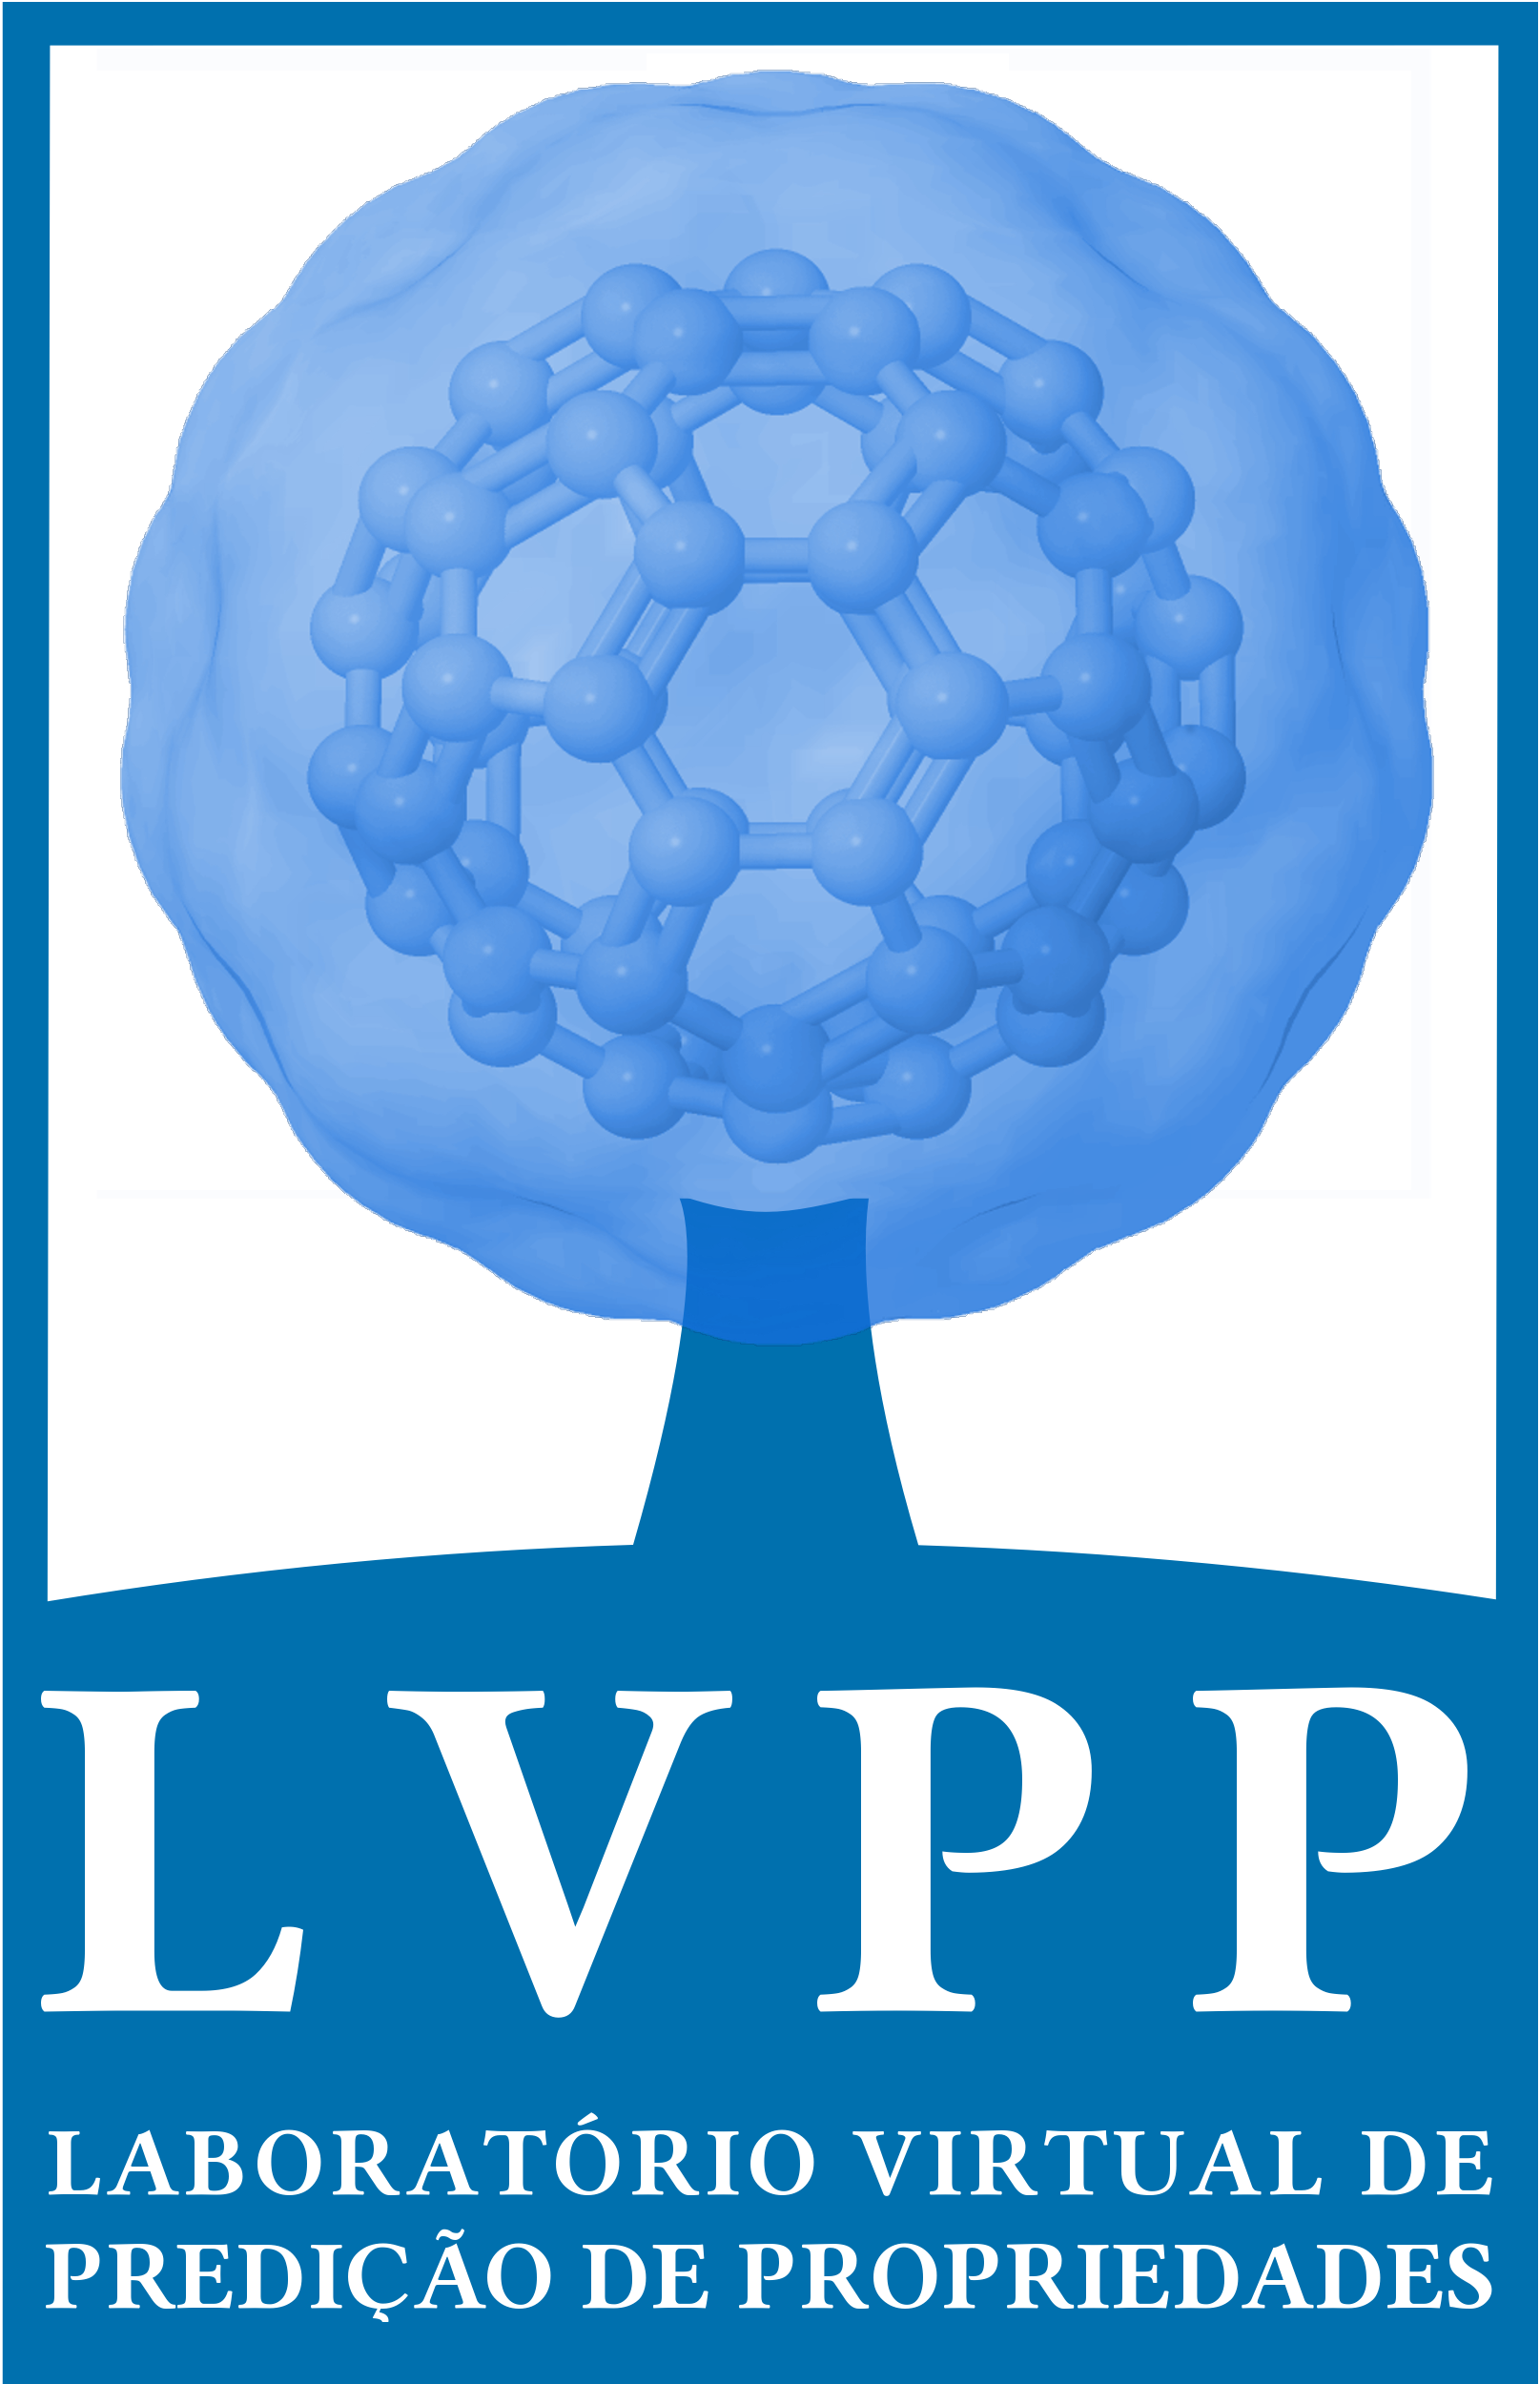
\includegraphics[width=0.9\textwidth]{LogoLVPP22}
\column{.7\textwidth}
\centering
FED. UNIV. OF RIO GRANDE DO SUL - BRAZIL \\
CHEMICAL ENGINEERING DEPARTMENT \\
LAB. VIRTUAL DE PREDI��O DE PROPRIEDADES \\
\url{http://www.enq.ufrgs.br/labs/lvpp}
\column{.2\textwidth}
\qrcodeonly{0.8}{http://www.enq.ufrgs.br/labs/lvpp}
\end{columns}
}

\begin{document}

\begin{vrpresentation}

\section{Introduction}


\begin{frame}
  \frametitle{Map}
\centering
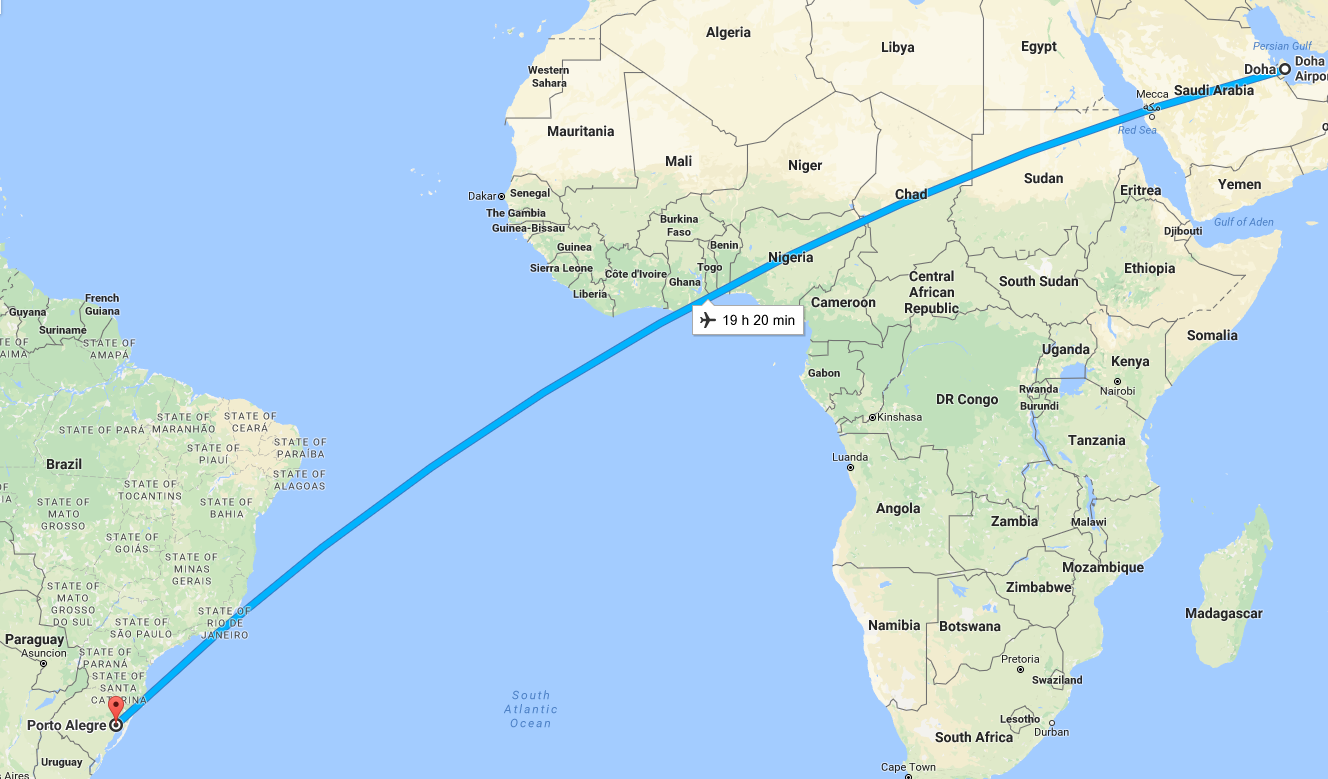
\includegraphics[width=0.8\textwidth]{Map}
\end{frame}

\begin{frame}
  \frametitle{Our Group: Virtual Laboratory for Property Predictions (LVPP)}
\centering
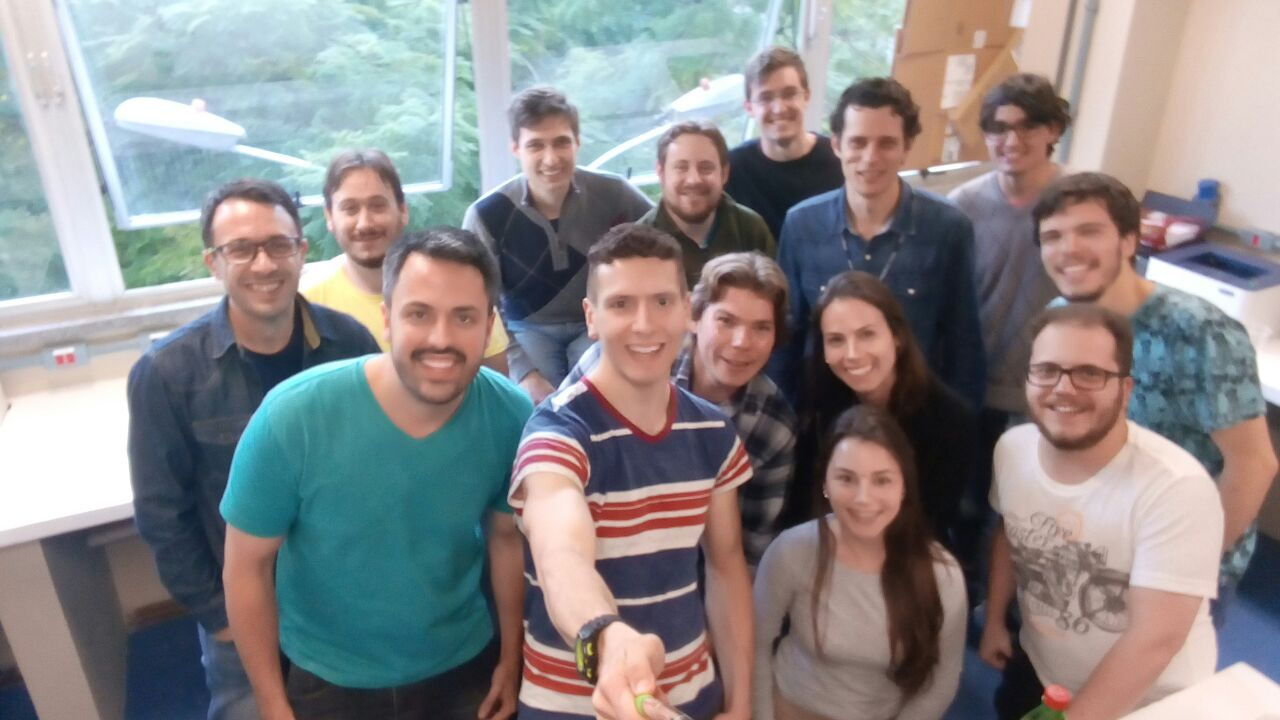
\includegraphics[width=0.8\textwidth]{Group}
\end{frame}

\subsection*{COSMO}


\begin{frame}[plain]
\frametitle{COSMO method (solutes alone)}
\begin{columns}[c]
\column{.2\textwidth}
\begin{center}
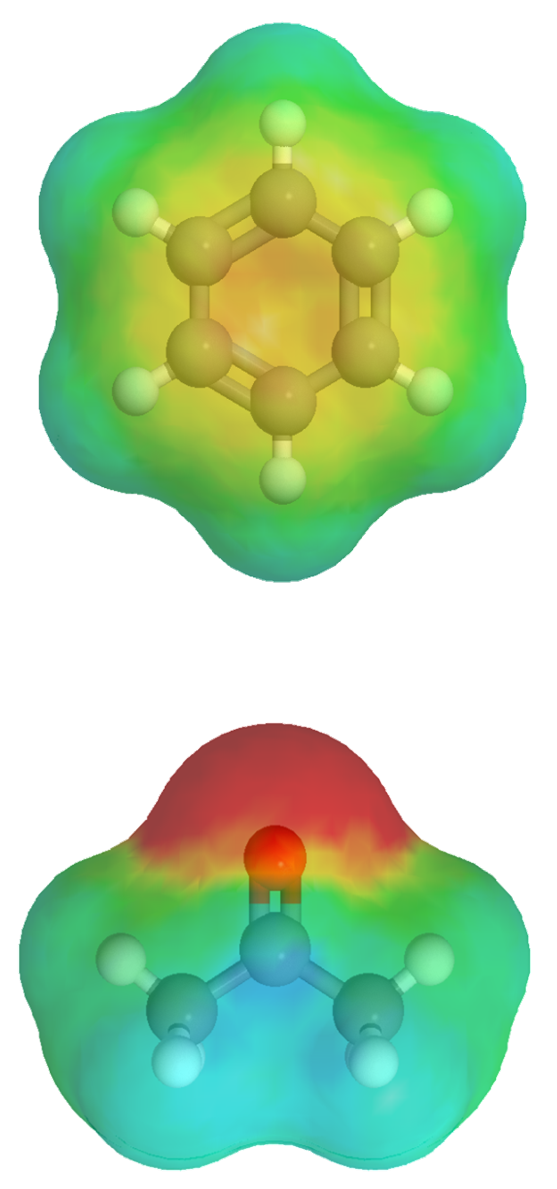
\includegraphics[width=\textwidth]{Figures/contato1}
\end{center}
\column{.8\textwidth}
\begin{itemize}
  \item The COSMO\footcite{Klamt1993} method was originally developed
  for the computation of solvation effects
    \item The method belongs to the class of dielectric continuum models\visible<2->{,
    the cavities are discretized into
   	\emph{segments} or \emph{patches}}
\end{itemize}
\visible<2->{
\begin{center}
\includegraphics[width=0.35\textwidth]{Figures/Chloroform.png}
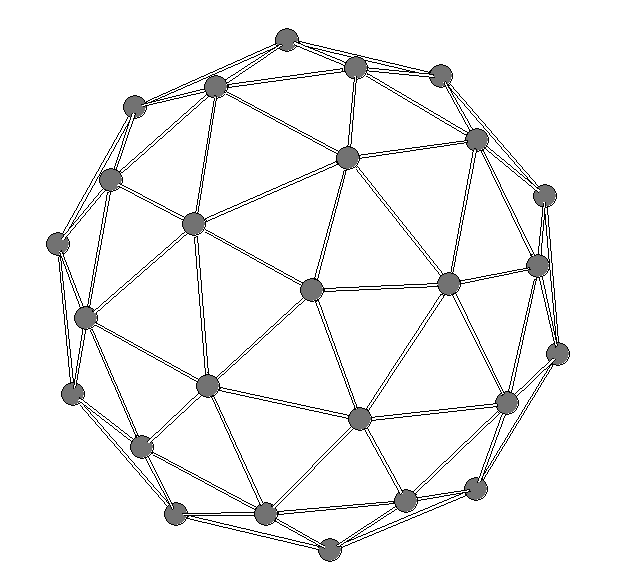
\includegraphics[width=0.25\textwidth]{Figures/AtomSegments.png}
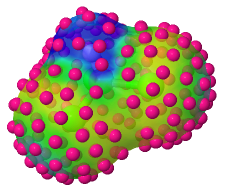
\includegraphics[width=0.35\textwidth]{Figures/ChloroformBalls.png}
\end{center}
}
\end{columns}
\end{frame}

\subsection*{COSMO-RS or COSMO-SAC}

\begin{frame}[plain]
\transdissolve
\frametitle{COSMO-RS -- Surface contacting theory (mixtures)}
\begin{columns}[c]
\column{.22\textwidth}
\begin{center}
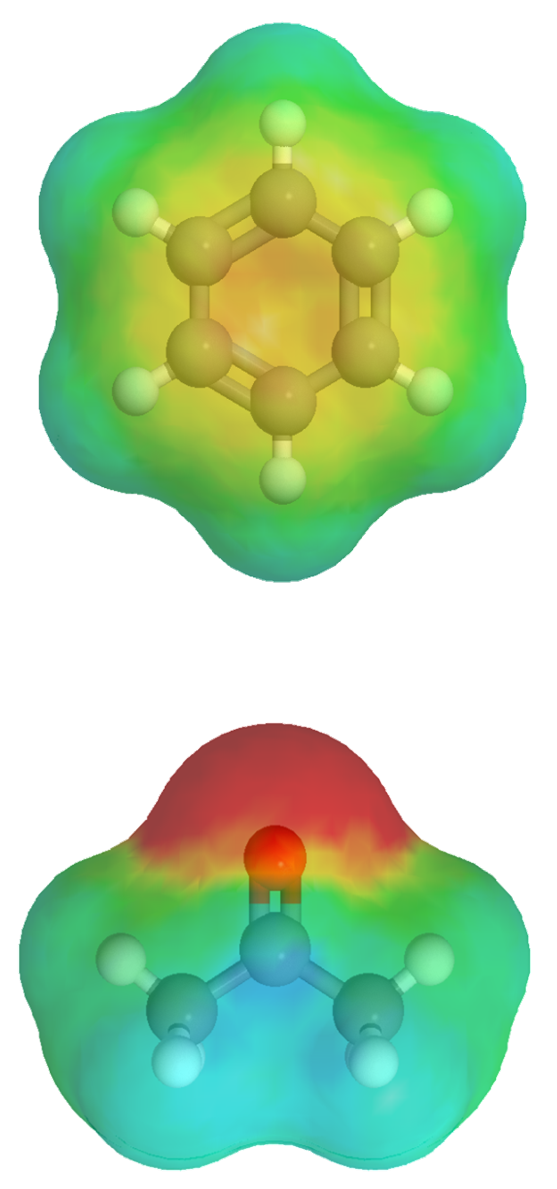
\includegraphics[width=\textwidth]{Figures/contato1}
\end{center}
\column{.22\textwidth}
\visible<2->{
\begin{center}
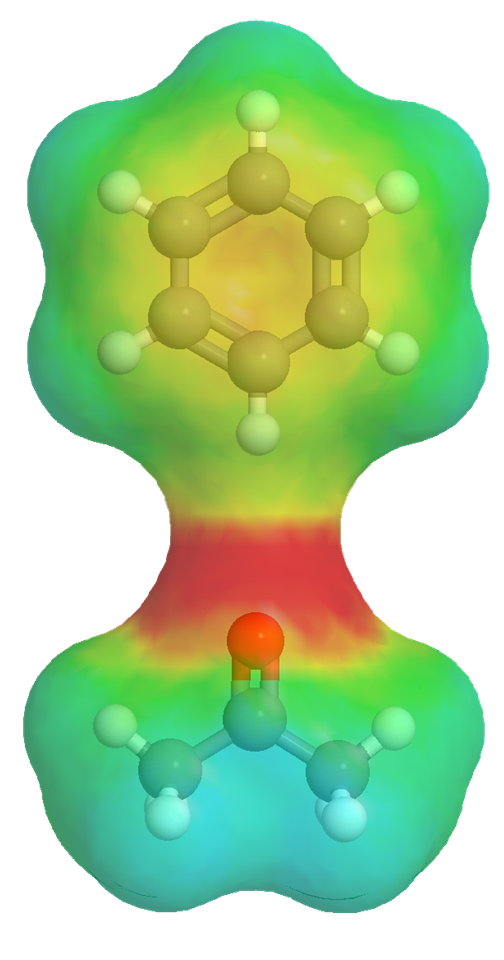
\includegraphics[width=\textwidth]{Figures/contato2}
\end{center}
}
\column{.55\textwidth}
\begin{itemize}
  \item In the COSMO-RS\myfootcitecol{Klamt1995} methods we rely
  	on COSMO computations \pause
    \item Based on these \emph{pure} substance computations, the mixture
    	behavior is predicted ($\gamma_i$)
   	\item The COSMO-SAC\myfootcitecol{Lin2002} formulation follows the same idea
\end{itemize}
\end{columns}
\end{frame}

\begin{frame}
\frametitle{COSMO-RS -- Surface contacting theory}
\begin{columns}[c]
\column{.3\textwidth}
\begin{center}
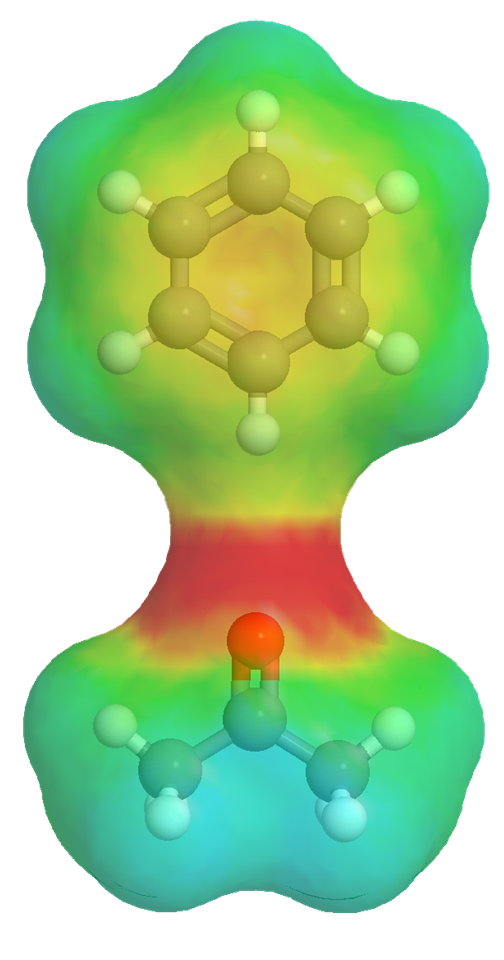
\includegraphics[width=0.8\textwidth]{Figures/contato2}
\end{center}

\column{.7\textwidth}
\begin{itemize}
    \item For each surface pair contact, there is an energy change
    \item This results in different behavior for different substances
    	in solution
    \item Clearly, there are many different possible contacting arranges
    and a \emph{statistical thermodynamics} treatment is necessary
    % \item For the F-SAC model, the COSMO-RS variant known as
    % COSMO-SAC\myfootcitecol{Lin2002} is used
\end{itemize}
\end{columns}
\end{frame}


\begin{frame}[plain]
\frametitle{COSMO-RS -- Surface contacting theory (mixtures)}

\begin{columns}[c]
\column{.6\textwidth}

\begin{itemize}
    \item Based on these \emph{pure} substance computations, the mixture
    	behavior is predicted ($\gamma_i$)
\end{itemize}

\centering
\includegraphics[width=0.4\textwidth]{Figures/chloroform}
\includegraphics[width=0.4\textwidth]{Figures/tetrahydrofuran}

\begin{itemize}
\scriptsize
\item ``It is always desirable to express the properties of a solution in terms that
can be calculated completely from the properties of the pure components.'' -- \fullcite{Prausnitz:1999}.
\end{itemize}

\column{.4\textwidth}
\centering
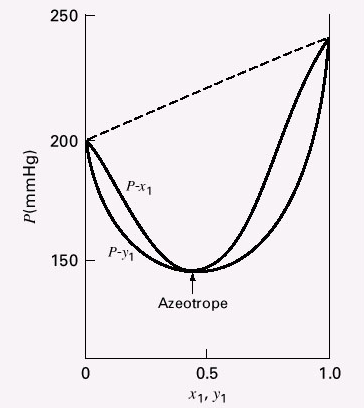
\includegraphics[width=\textwidth]{Figures/NegativeDeviation}\\
\scriptsize
Chloroform/tetrahydrofuran at 30$^\circ$C
\end{columns}
\end{frame}


\subsection*{Sigma profile}
 
\begin{frame}
\frametitle{Sigma profile -- $p(\sigma)$}
\begin{columns}[c]
\column{.45\textwidth}
\begin{center}
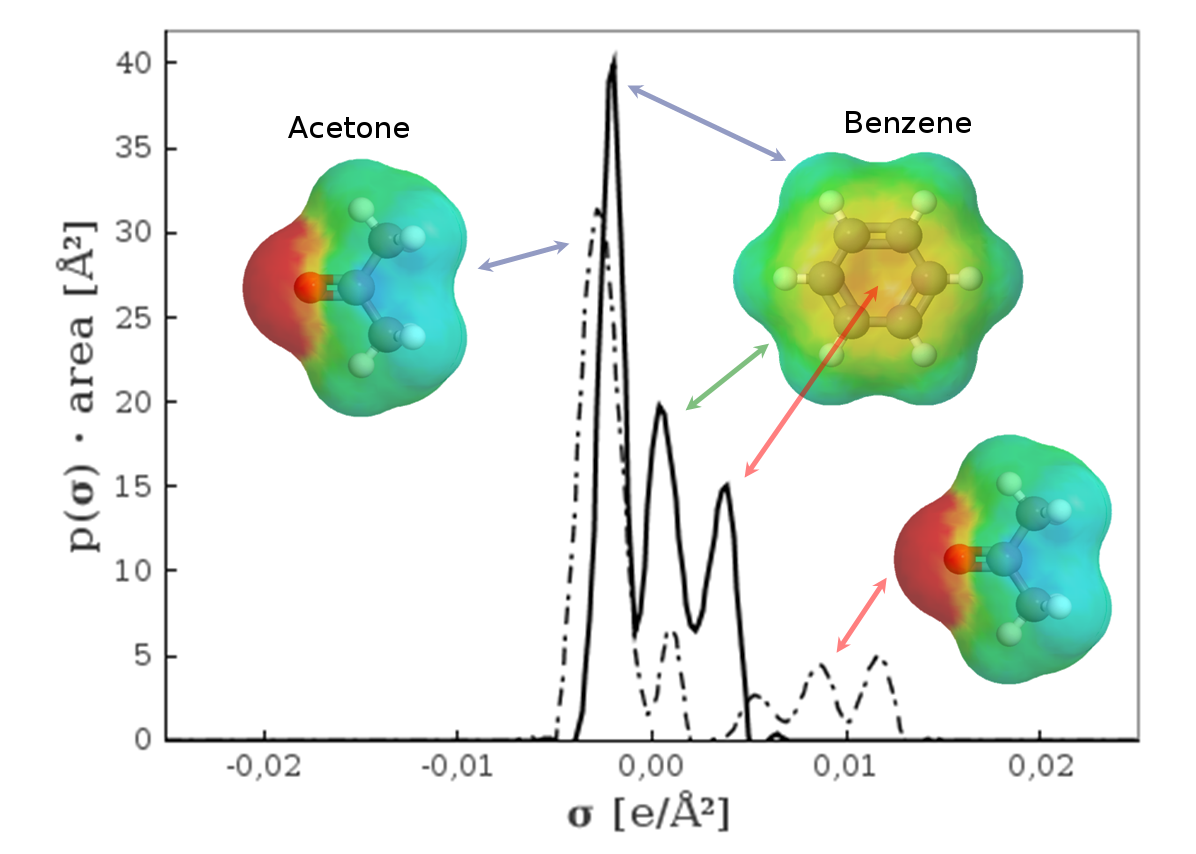
\includegraphics[width=\textwidth]{Figures/perfilsigma} \\
\begin{tikzpicture}
    \shade[opacity=0](0,0) rectangle (0.6cm,0.3cm);
    \shade[left color=blue,right color=green](0.6cm,0) rectangle (3.2cm,0.3cm);
    \shade[left color=green,right color=red](3.2cm,0) rectangle (6cm,0.3cm);
\end{tikzpicture}
\end{center}
\column{.45\textwidth}
\begin{itemize}
    \item For a statistical thermodynamics treatment (without using MD),
    	the 3D apparent surface charges are projected into a simple histogram
    \item These \textbf{pure compound} distributions, known as \emph{sigma profiles} -- $p(\sigma)$,
    	are the basis for computing the activity coefficients in \textbf{mixture}
\end{itemize}
\end{columns}
\pause
\scriptsize
\begin{itemize}
\item ``It is always desirable to express the properties of a solution in terms that
can be calculated completely from the properties of the pure components.'' -- \fullcite{Prausnitz:1999}.
\end{itemize}
\end{frame}

\section{Some Challenges}

% \begin{frame}
% \frametitle{Some challenges for COSMO-based models}
% \begin{enumerate}
%     \item Sigma profile database
%     \item Reliability
%     \item Computational cost
% %    \item Wide range of temperature and pressure
% \end{enumerate}
% \end{frame}

\subsection*{Sigma profile database}

\begin{frame}
  \frametitle{Sigma profile database}
  \begin{columns}[c]
\column{.2\textwidth}
\begin{center}
\includegraphics[width=\textwidth]{Figures/Chloroform}
\end{center}
\column{.8\textwidth}
\begin{itemize}
    \item The quantum chemistry calculations for generating the sigma profiles
    represent the most time-consuming aspect
    of COSMO-based methods \pause
    \item There are several different quantum chemistry packages implementing
    the COSMO method, \emph{e.g.}: Gaussian, Turbomole, MOPAC, DMol3 and GAMESS.
    \item However, different packages lead to different sigma profiles
    \myfootcitecol{Mullins2006}, requiring specific model parametrizations
    \myfootcitecol{Gerber:2013}
\end{itemize}
\end{columns}
\end{frame}

\begin{frame}
  \frametitle{VT-2005 database}
  \begin{columns}[c]
\column{.2\textwidth}
\begin{center}
\includegraphics[width=\textwidth]{Figures/Chloroform}
\end{center}
\column{.8\textwidth}
\begin{itemize}
    \item The freely available database known as VT-2005 contains 1432
    compounds\myfootcitecol{Mullins2006}, mostly solvents and small molecules
    \item The VT-2006 contains 206 pharmaceutical-related molecules \pause
    \item VT-databases were constructed using DMol3 (Materials Studio) which
    is very expensive\ldots
\end{itemize}
\end{columns}
\end{frame}

\begin{frame}
  \frametitle{Alternatives available}
  \begin{columns}[c]
\column{.2\textwidth}
\begin{center}
\includegraphics[width=\textwidth]{Figures/Chloroform}
\end{center}
\column{.8\textwidth}
\begin{itemize}
    \item Alternative database with nearly 1000 compounds\myfootcitecol{Gerber:2010}
    using MOPAC (semi-empirical -- could lead to poor results)\pause
    \item GAMESS (freely available, including source code) can be
    used\myfootcitecol{Wang200937} \pause
\end{itemize}
\end{columns}

\begin{exampleblock}{Suggestion}
Assemble an extensive and freely available database using the rigorous methods
available in GAMESS
\end{exampleblock}
\end{frame}

\subsection*{Reliability}

\begin{frame}
  \frametitle{Reliability: The good\ldots}
  There are several very good results in the literature, for instance
  \fullcite{Paulechka2015}
  \begin{center}
  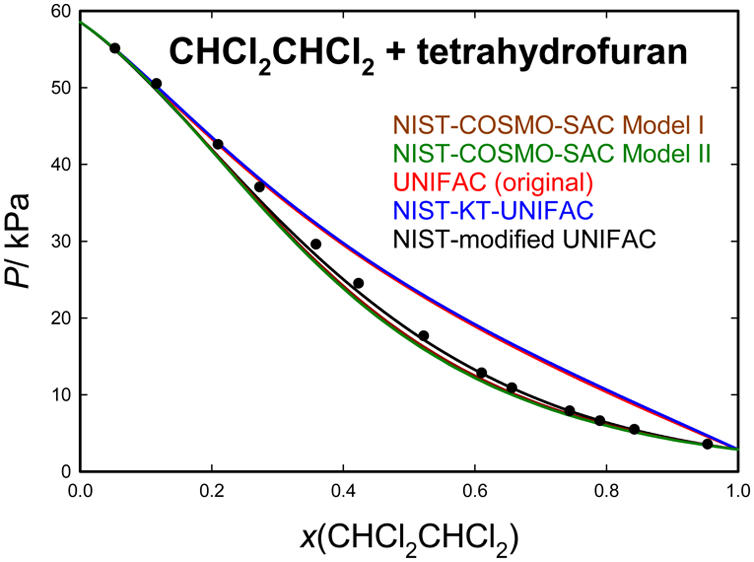
\includegraphics[width=0.5\textwidth]{Figures/GoodResult}
  \end{center}
\end{frame}

\begin{frame}
  \frametitle{The good, the bad and the ugly\ldots}
  There are also bad and ugly results around, \emph{e.g.}
  \fullcite{Grensemann2005}, for acetone(1)/diisopro-pylether and
  perfluorohexane(1)/\emph{n}-hexane, respectivelly:
  \begin{center}
  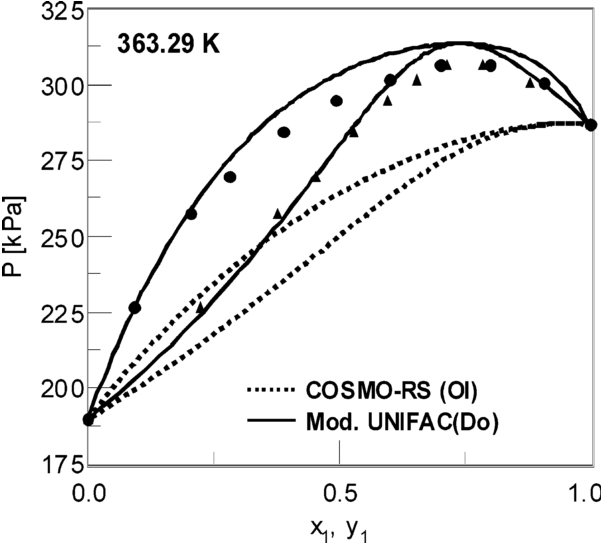
\includegraphics[width=0.4\textwidth]{Figures/BadResult}
  \hspace{0.5cm}
  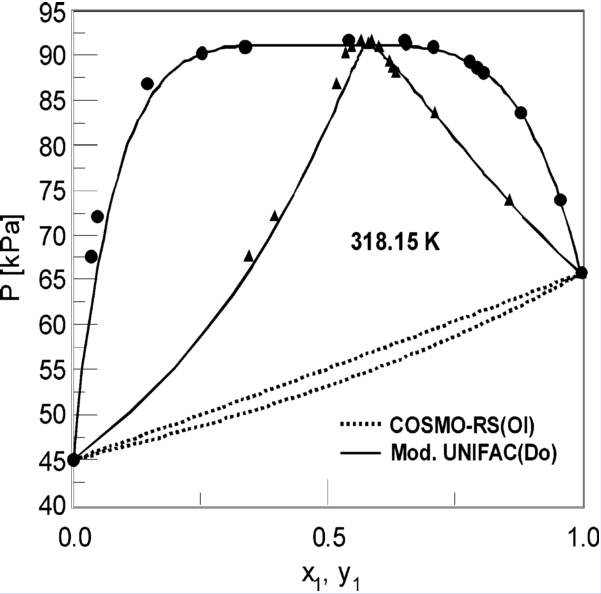
\includegraphics[width=0.4\textwidth]{Figures/UglyResult}
  \end{center}
\end{frame}


\begin{frame}
  \frametitle{Precision of COSMO-based models}
  \begin{itemize}
    \item COSMO-based models have exceptional theoretical features
    \item However, very often empirical modifications are needed for improving the agreement with
    	experimental data, for instance:
    	\begin{itemize}
    	  \item Corrections in the water apparent surface charge \myfootcite{Grensemann:2005}
    	  \item Empirical scaling factors \myfootcite{Gerber:2010}
    	  	or empirically scaled surface areas \myfootcite{Reinisch:2011}
    	  \item Special parametrizations for different families, \emph{e.g.} alcohols\myfootcite{Franke2012}
    	  \item \ldots
	\end{itemize}
  \end{itemize}
\end{frame}


\begin{frame}
\frametitle{F-SAC: Functional-Segment Activity Model}
\transdissolve
\begin{columns}[c]
\column{.5\textwidth}
\begin{center}
  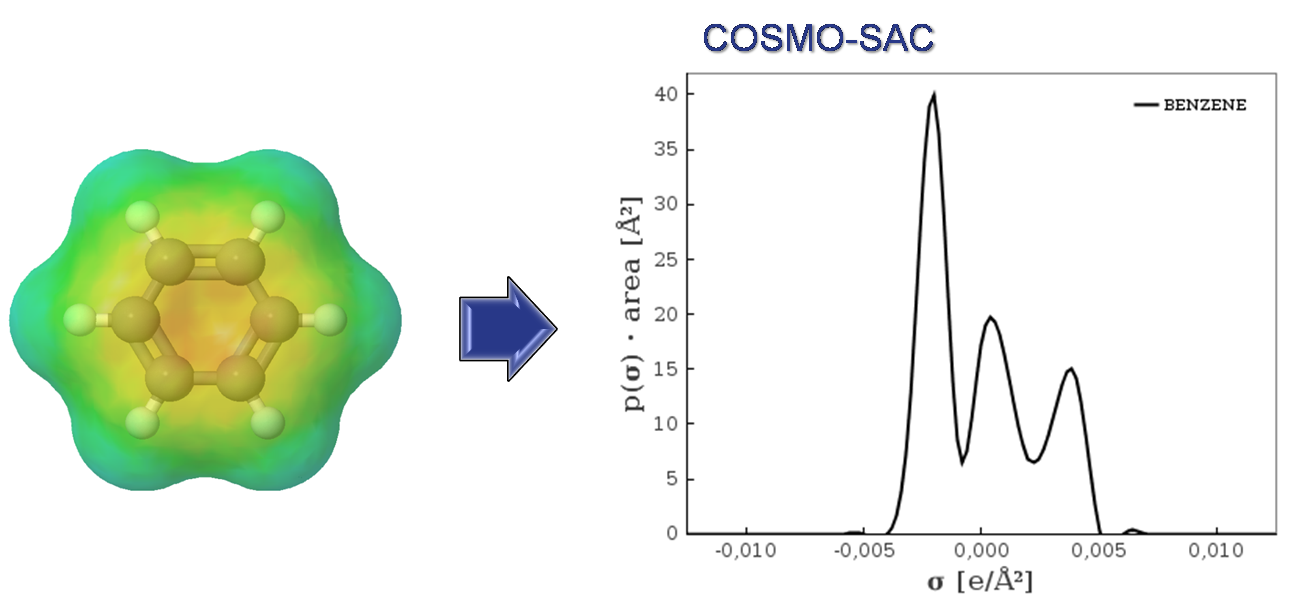
\includegraphics[width=\textwidth]{Figures/perfil1}\\ 
  \visible<2->{
  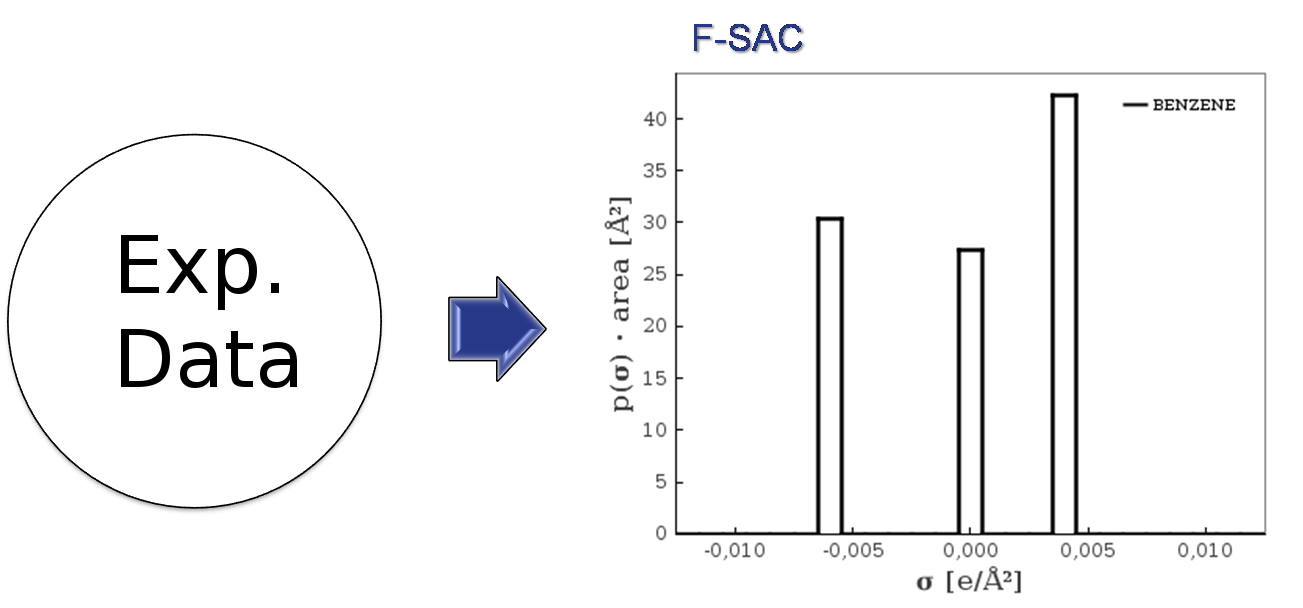
\includegraphics[width=\textwidth]{Figures/perfil2}
  }
\end{center}
\column{.5\textwidth}
\pause
\begin{itemize}
  \item In the F-SAC model, the quantum chemistry computation
  	is replaced by an artificial sigma-profile\myfootcitecol{SoaresFSAC1}
  \item Reduced predictive power
  \item But \textbf{hopefully, with increased resolution}
  	and with less parameters than UNIFAC-type models
\end{itemize}
\end{columns}
\end{frame}

\begin{frame}
\frametitle{F-SAC: Functional-Segment Activity Model}
\begin{itemize}
  	\item F-SAC and COSMO-SAC model equations are identical, the difference is in
  		the sigma profile
    % \item �rea superficial dos grupos � id�ntica
    \item In the F-SAC model there is a neutral and two charged peaks per functional group 
    \item Simply add the sigma-profiles of functional groups to get the sigma-profile of molecules
\end{itemize}
\begin{center}
  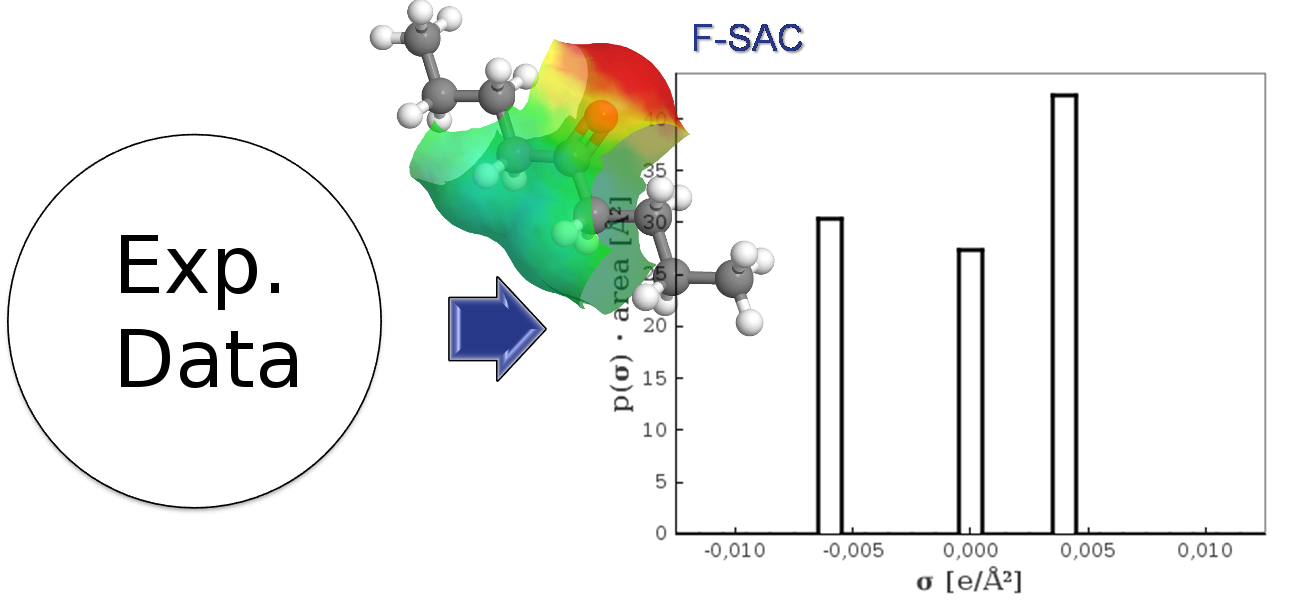
\includegraphics[width=0.65\textwidth]{Figures/perfil3}
\end{center}
\end{frame}

\begin{frame}[plain]
  \frametitle{Why don't just use UNIFAC instead?}
  \begin{center}
  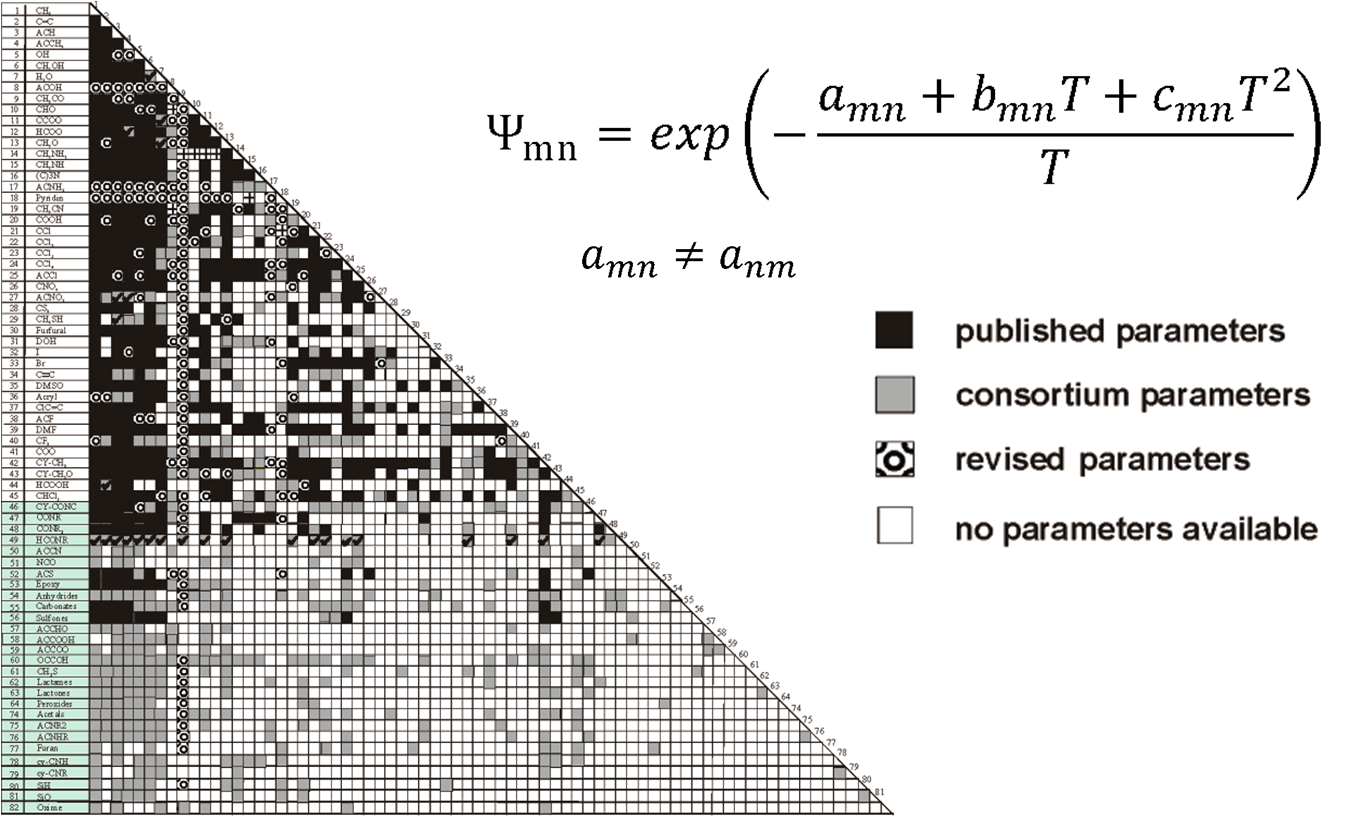
\includegraphics[width=0.7\textwidth]{Figures/unifac}
  \end{center}
  According to UNIFAC (Do) revision 5 -- \fullcite{Jakob2006}.
  
\end{frame}

\begin{frame}
\frametitle{F-SAC parameters}
\begin{columns}
\column{.7\textwidth}
  \begin{itemize}
    \item For the \textbf{24 grupos} considered, only \textbf{152} parameters were calibrated.
    \item Only the hydrogen-bonding$^\star$ energies are \textbf{pairwise}
    \item All other parameters are for \textbf{pure} groups alone, reducing the
    	total number of parameters
    \item In order to represent the same molecules in mixtures, \textbf{778} parameters are used in UNIFAC~(Do).
  \end{itemize}
\column{.3\textwidth}
  \begin{center}
  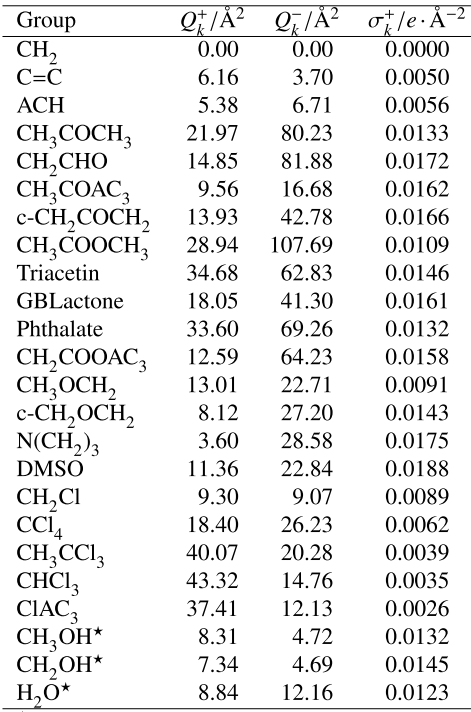
\includegraphics[width=\textwidth]{Figures/parsFSAC}
  \end{center}
\end{columns}
\end{frame}

\begin{frame}
  \frametitle{VLE predictions for non-associating mixtures}
  
\begin{figure}
\centering
\subfigure[Chloroform/n-heptane]
{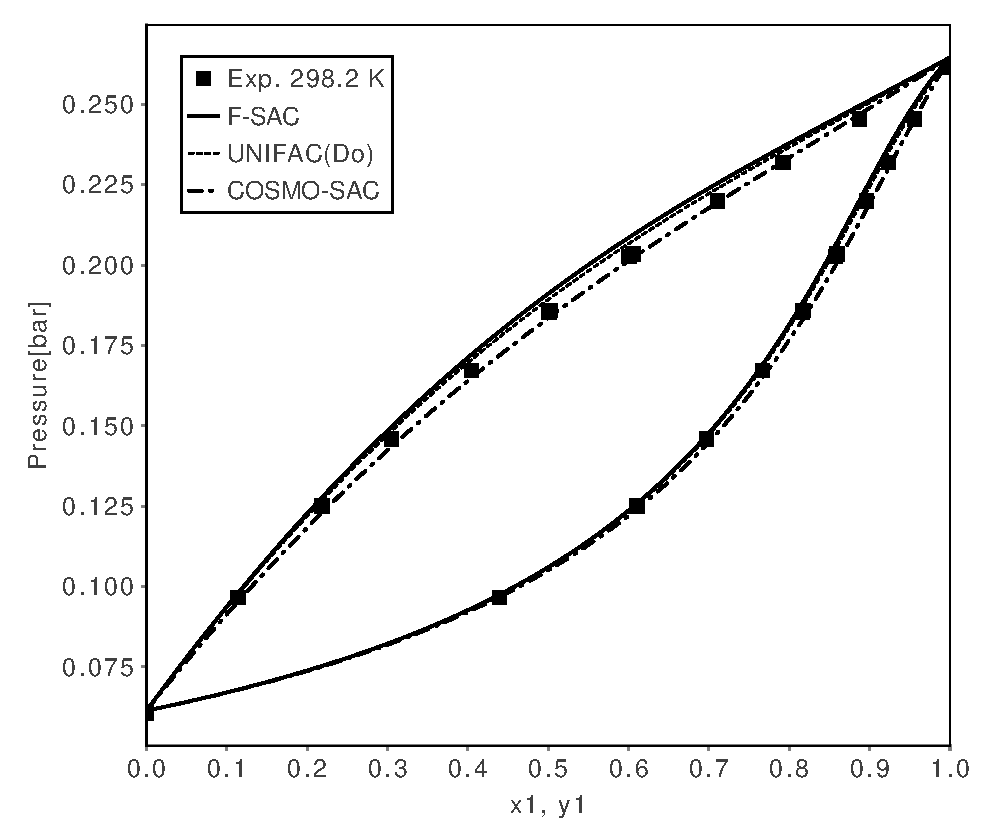
\includegraphics[width=0.4\textwidth]{Figures/CHLOROFORM-N-HEPTANE}}
\subfigure[Acetone/cyclohexane]
{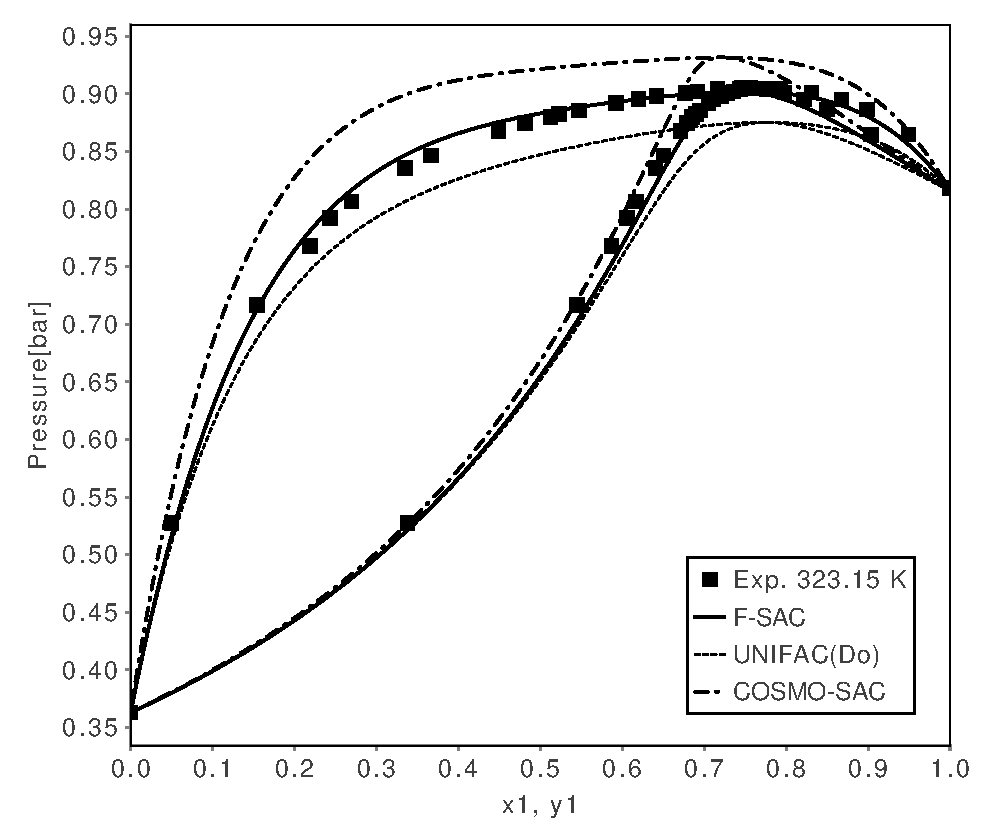
\includegraphics[width=0.4\textwidth]{Figures/ACETONE-CYCLOHEXANE.pdf}}
\end{figure}
\scriptsize
\fullcite{SoaresFSAC1}
\end{frame}


\begin{frame}
  \frametitle{VLE predictions for non-associating mixtures}
\begin{figure}
\centering
\subfigure[Dimethyl ether/1-butene] {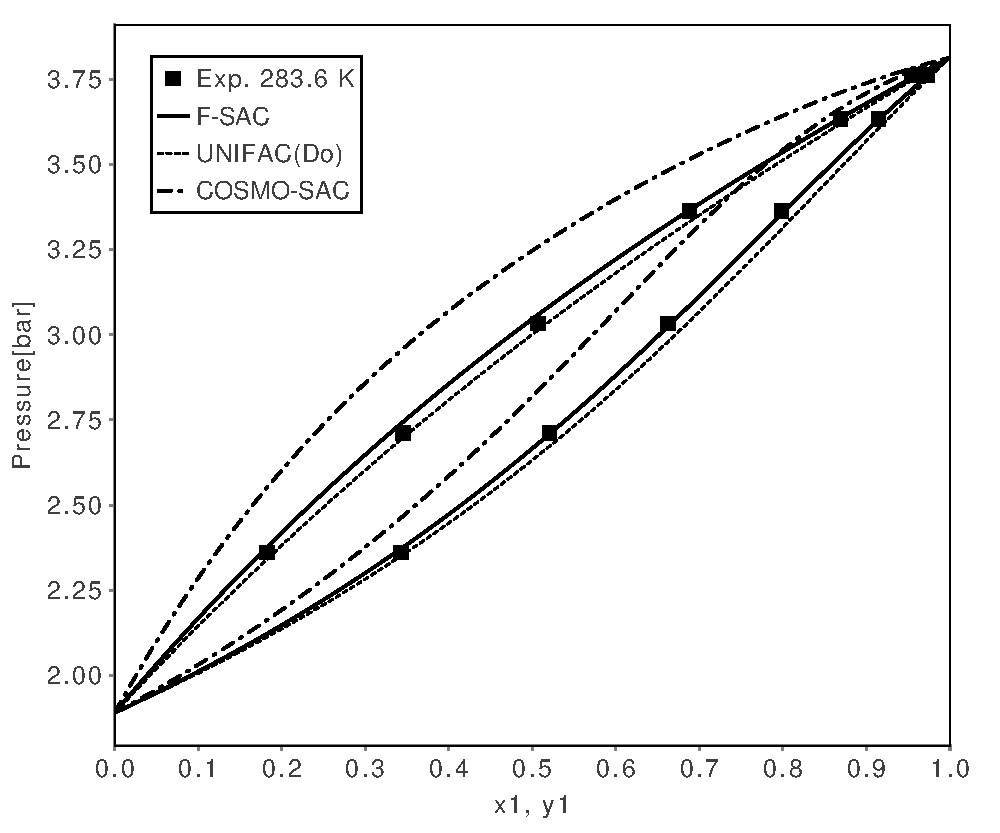
\includegraphics[width=0.4\textwidth]{Figures/DIMETHYL_ETHER-1-BUTENE.pdf}}
\subfigure[Methyl acetate/1-hexene] {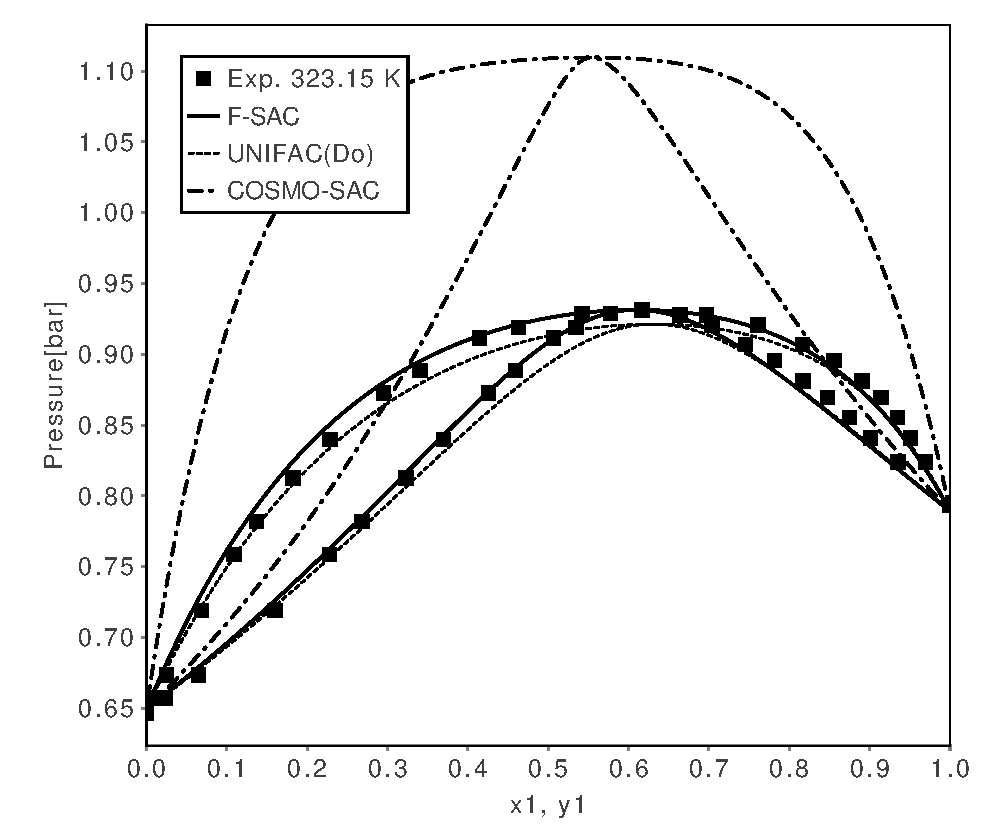
\includegraphics[width=0.4\textwidth]{Figures/METHYL_ACETATE-1-HEXENE}}
\end{figure}
\scriptsize
\fullcite{SoaresFSAC1}
\end{frame}

\begin{frame}
\frametitle{F-SAC parameters for Hydrogen-Bonding mixtures (association)}

\begin{itemize}
  \item HB-acceptor is red (positive), HB-donor is blue (negative)\footfullcite{SoaresFSAC2} 
\end{itemize}

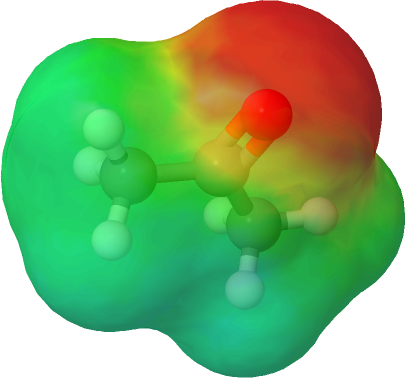
\includegraphics[width=0.2\textwidth]{Figures/ACETONE}
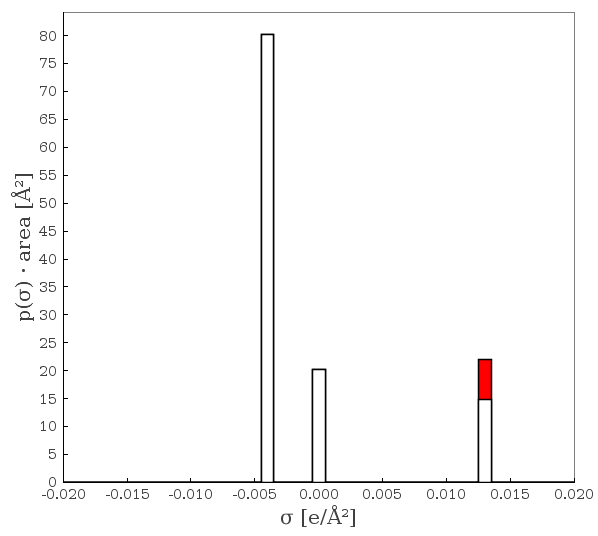
\includegraphics[width=0.25\textwidth]{Figures/FSAC-HB-ACETONE}
\hspace{1cm}
\includegraphics[width=0.2\textwidth]{Figures/CHLOROFORM}
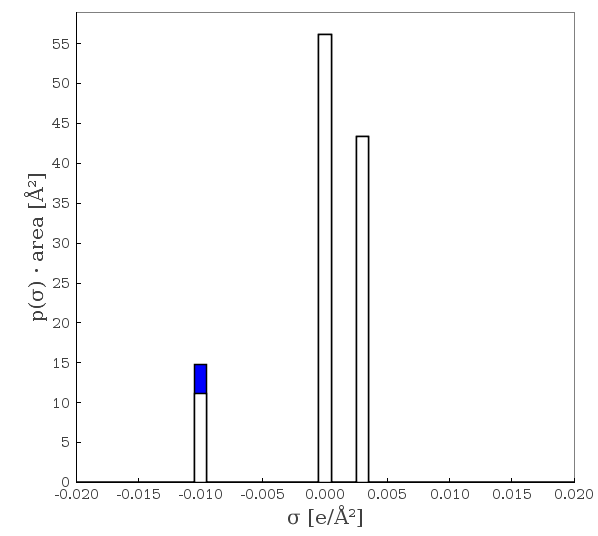
\includegraphics[width=0.25\textwidth]{Figures/FSAC-HB-CHLOROFORM}

%  \tikzoverlay[] at (0.2\textwidth,0.1cm) {
%  \qrcodedoi{0.8}{10.1021/ie4013979}
%  };
\end{frame}

 
\begin{frame}
  \frametitle{VLE predictions for associating mixtures}
\begin{figure}
\centering
\subfigure[diethyl-ether/chloroform]{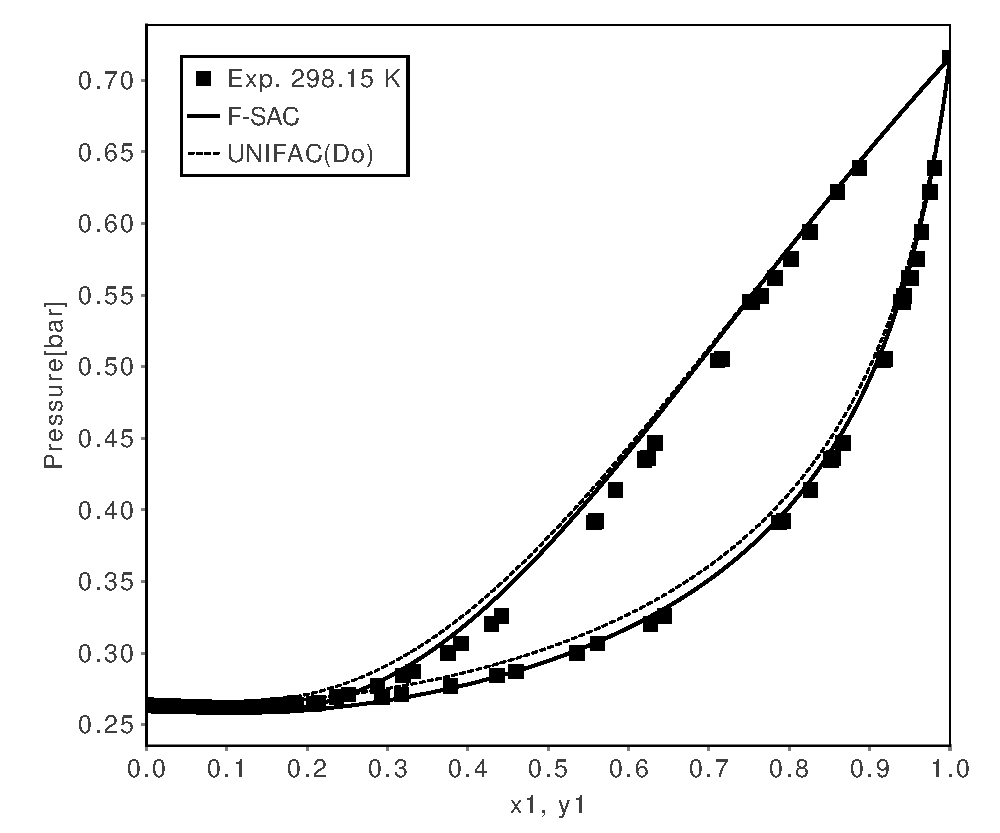
\includegraphics[width=0.4\textwidth]{Figures/DIETHYL_ETHER-CHLOROFORM}}
\subfigure[toluene/3-methyl,1-butanol]{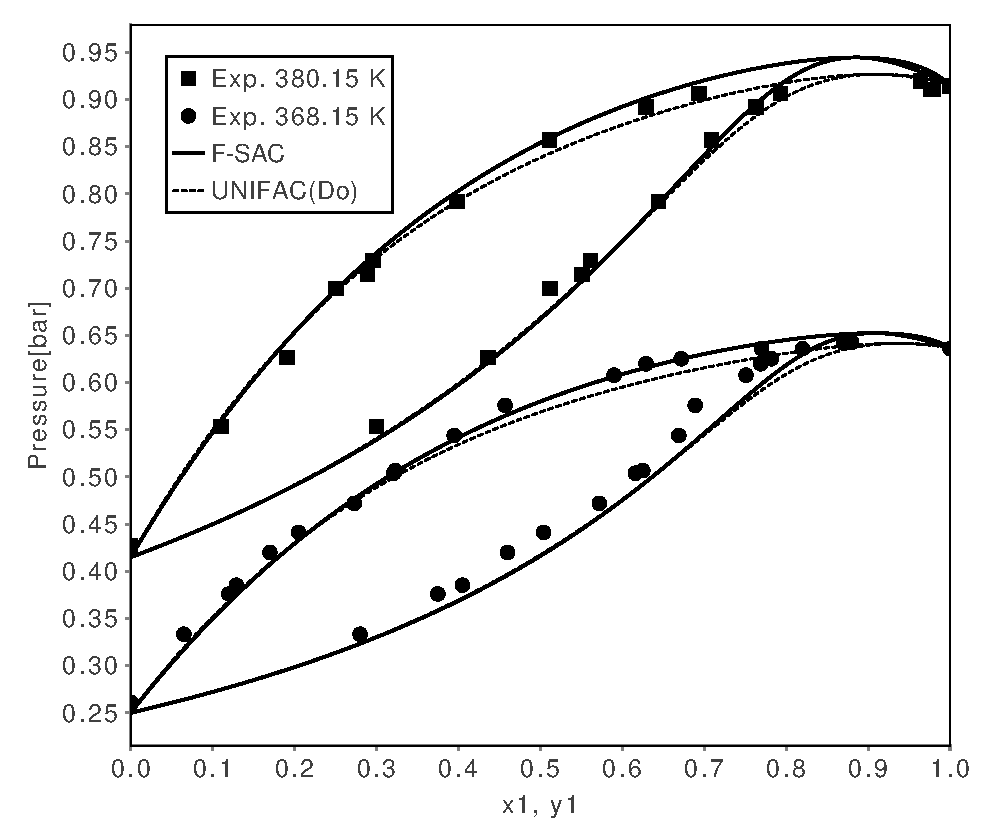
\includegraphics[width=0.4\textwidth]{Figures/TOLUENE-3-METHYL-1-BUTANOL}}
\end{figure}
\scriptsize
\fullcite{SoaresFSAC2}
\end{frame}

\begin{frame}
  \frametitle{IDAC comparison for associating mixtures (water excluded)}

\begin{figure}
\subfigure[F-SAC] {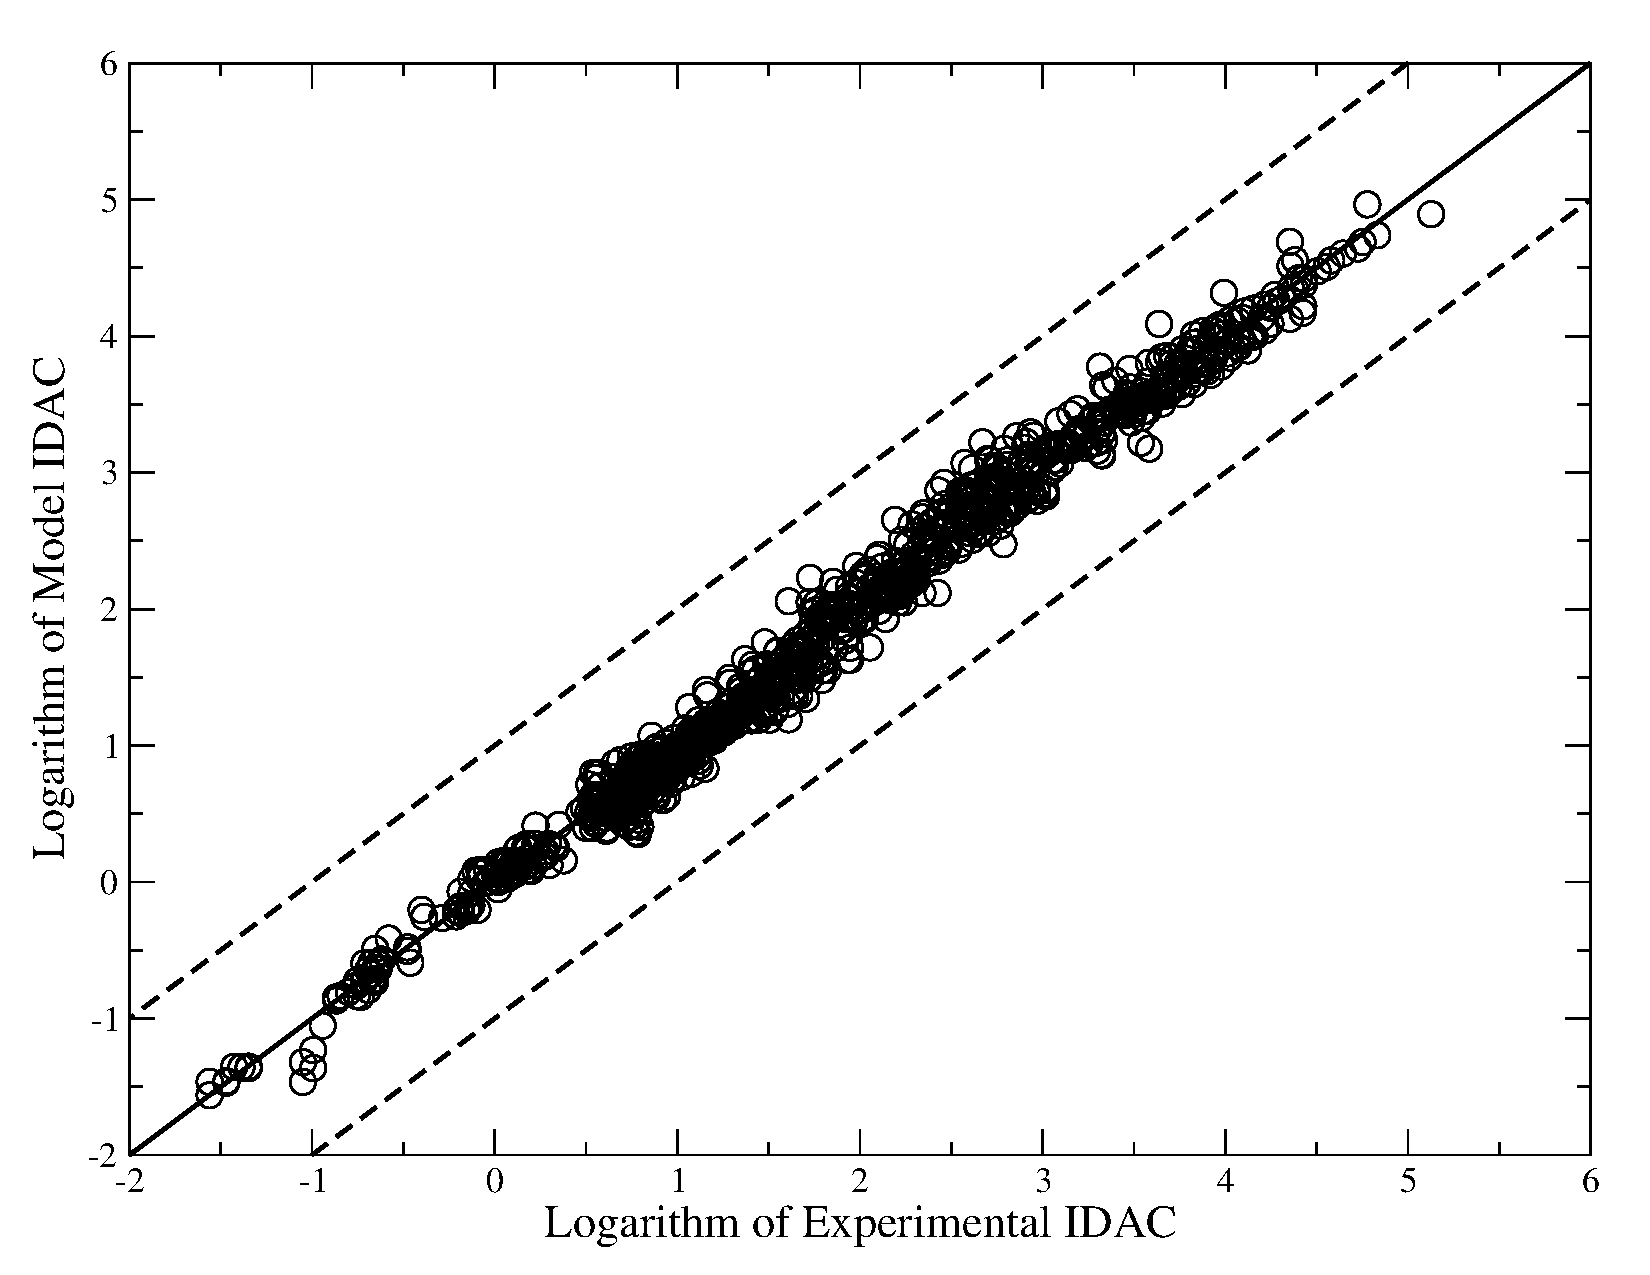
\includegraphics[width=0.4\textwidth]{Figures/IDACHB_fsac}}
\subfigure[UNIFAC~(Do)] {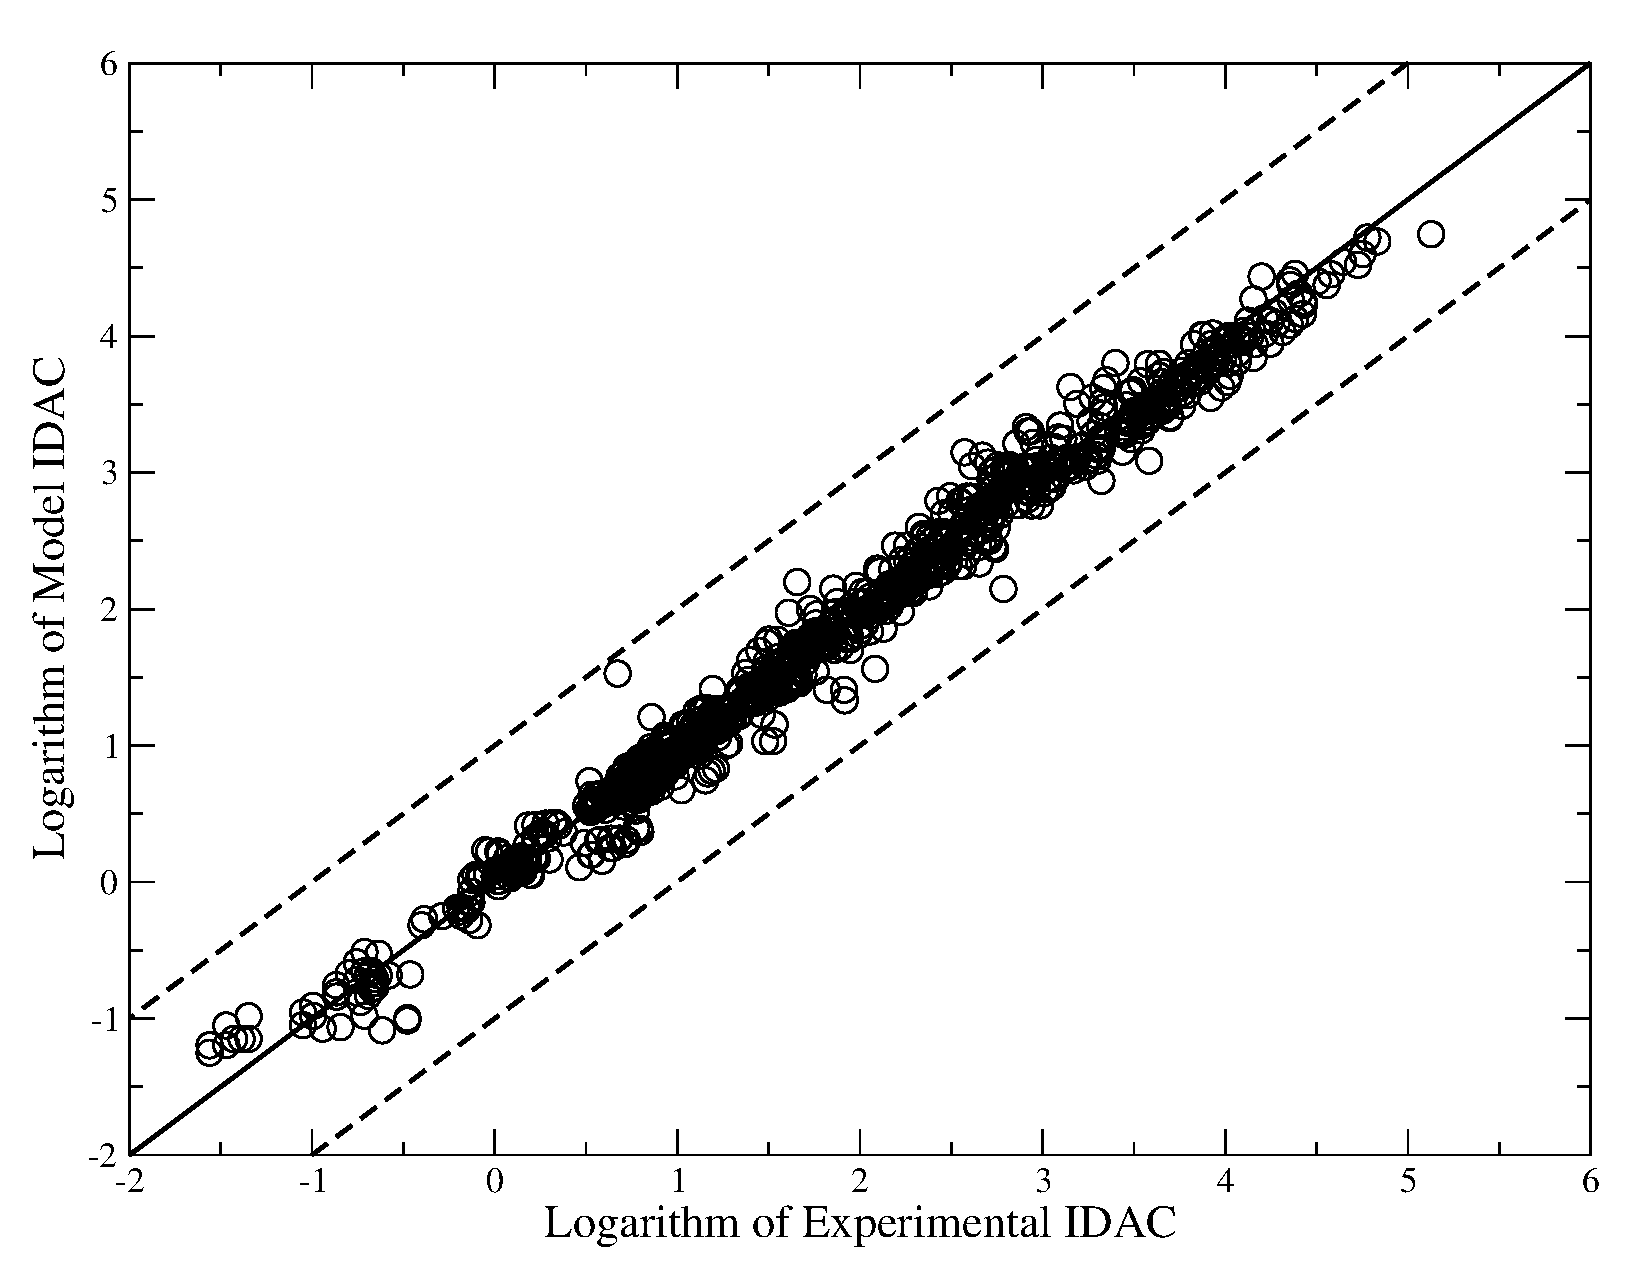
\includegraphics[width=0.4\textwidth]{Figures/IDACHB_unifac}}
\end{figure}
\scriptsize
\fullcite{SoaresFSAC2}
\end{frame}

\begin{frame}
  \frametitle{IDAC comparison for mixtures with water}

\begin{figure}
\subfigure[F-SAC] {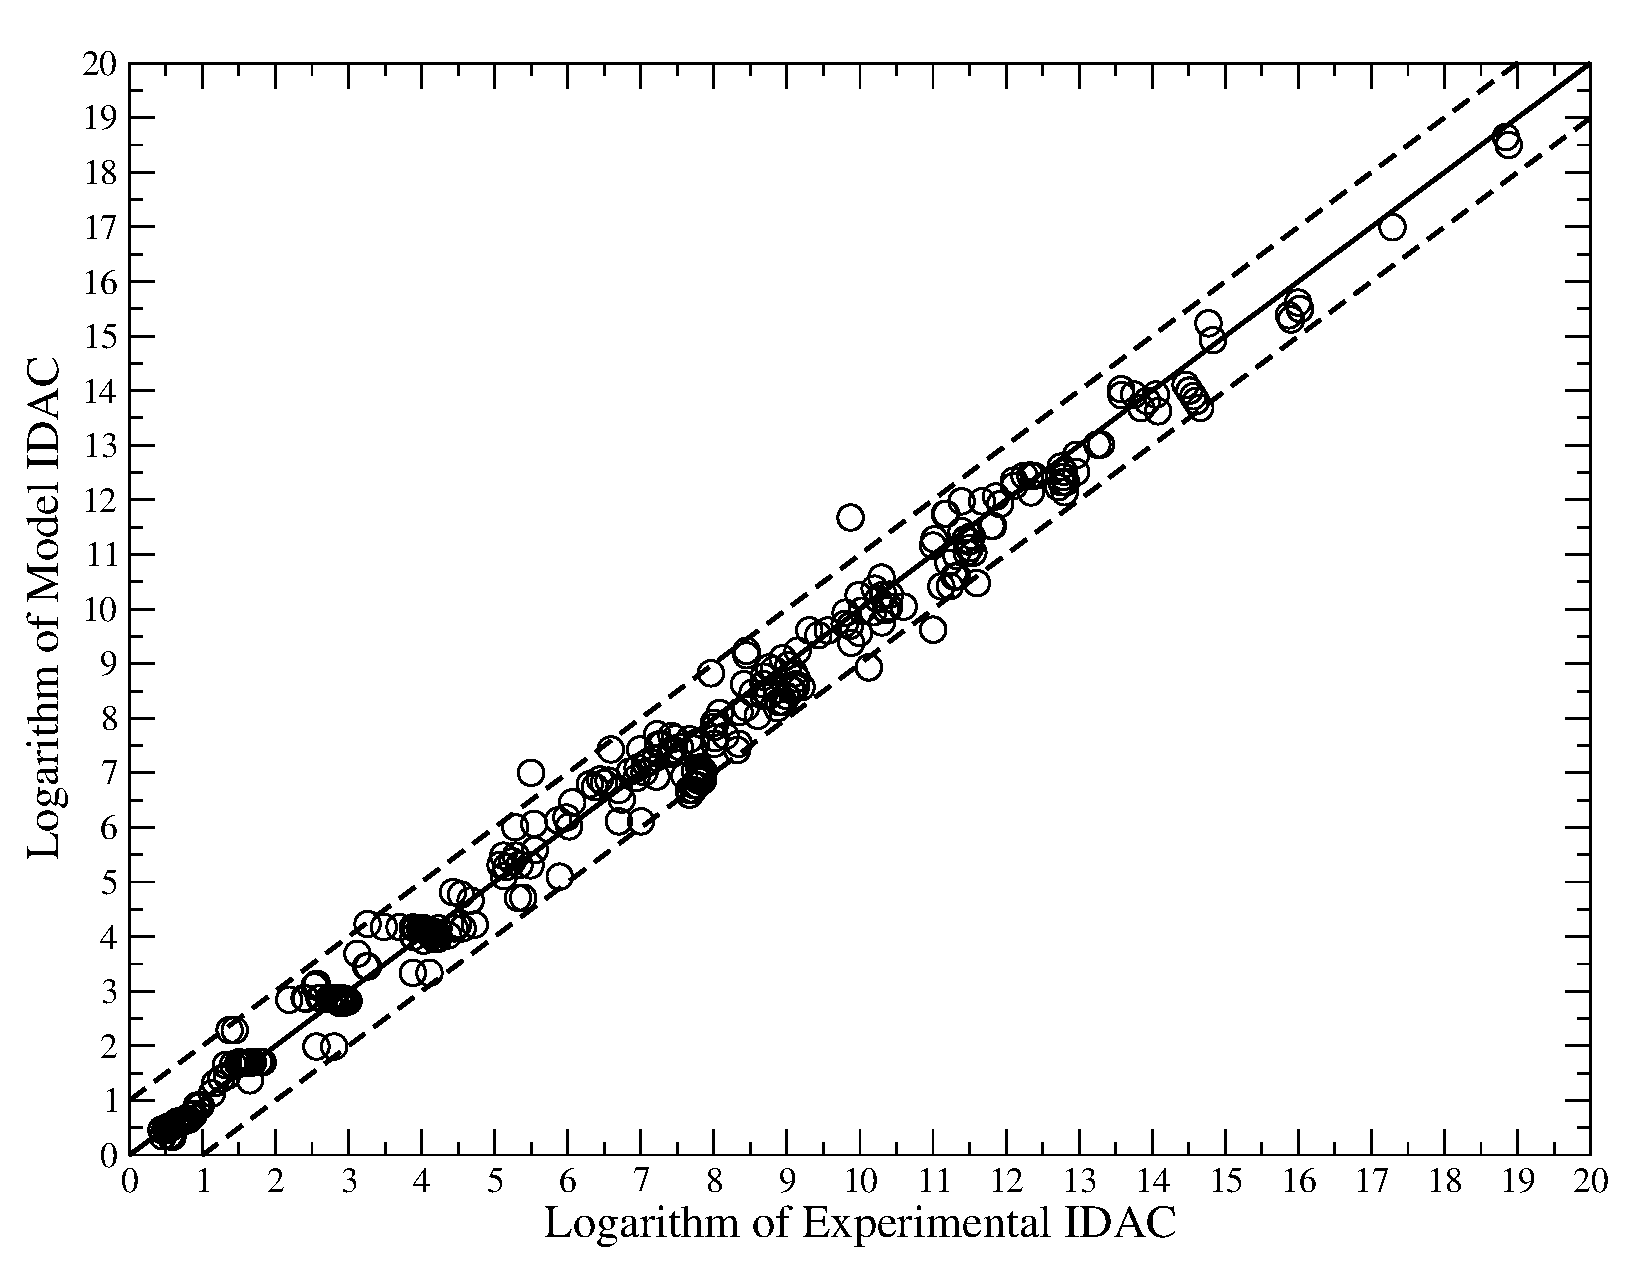
\includegraphics[width=0.4\textwidth]{Figures/IDACAq_fsac}}
\subfigure[UNIFAC~(Do)] {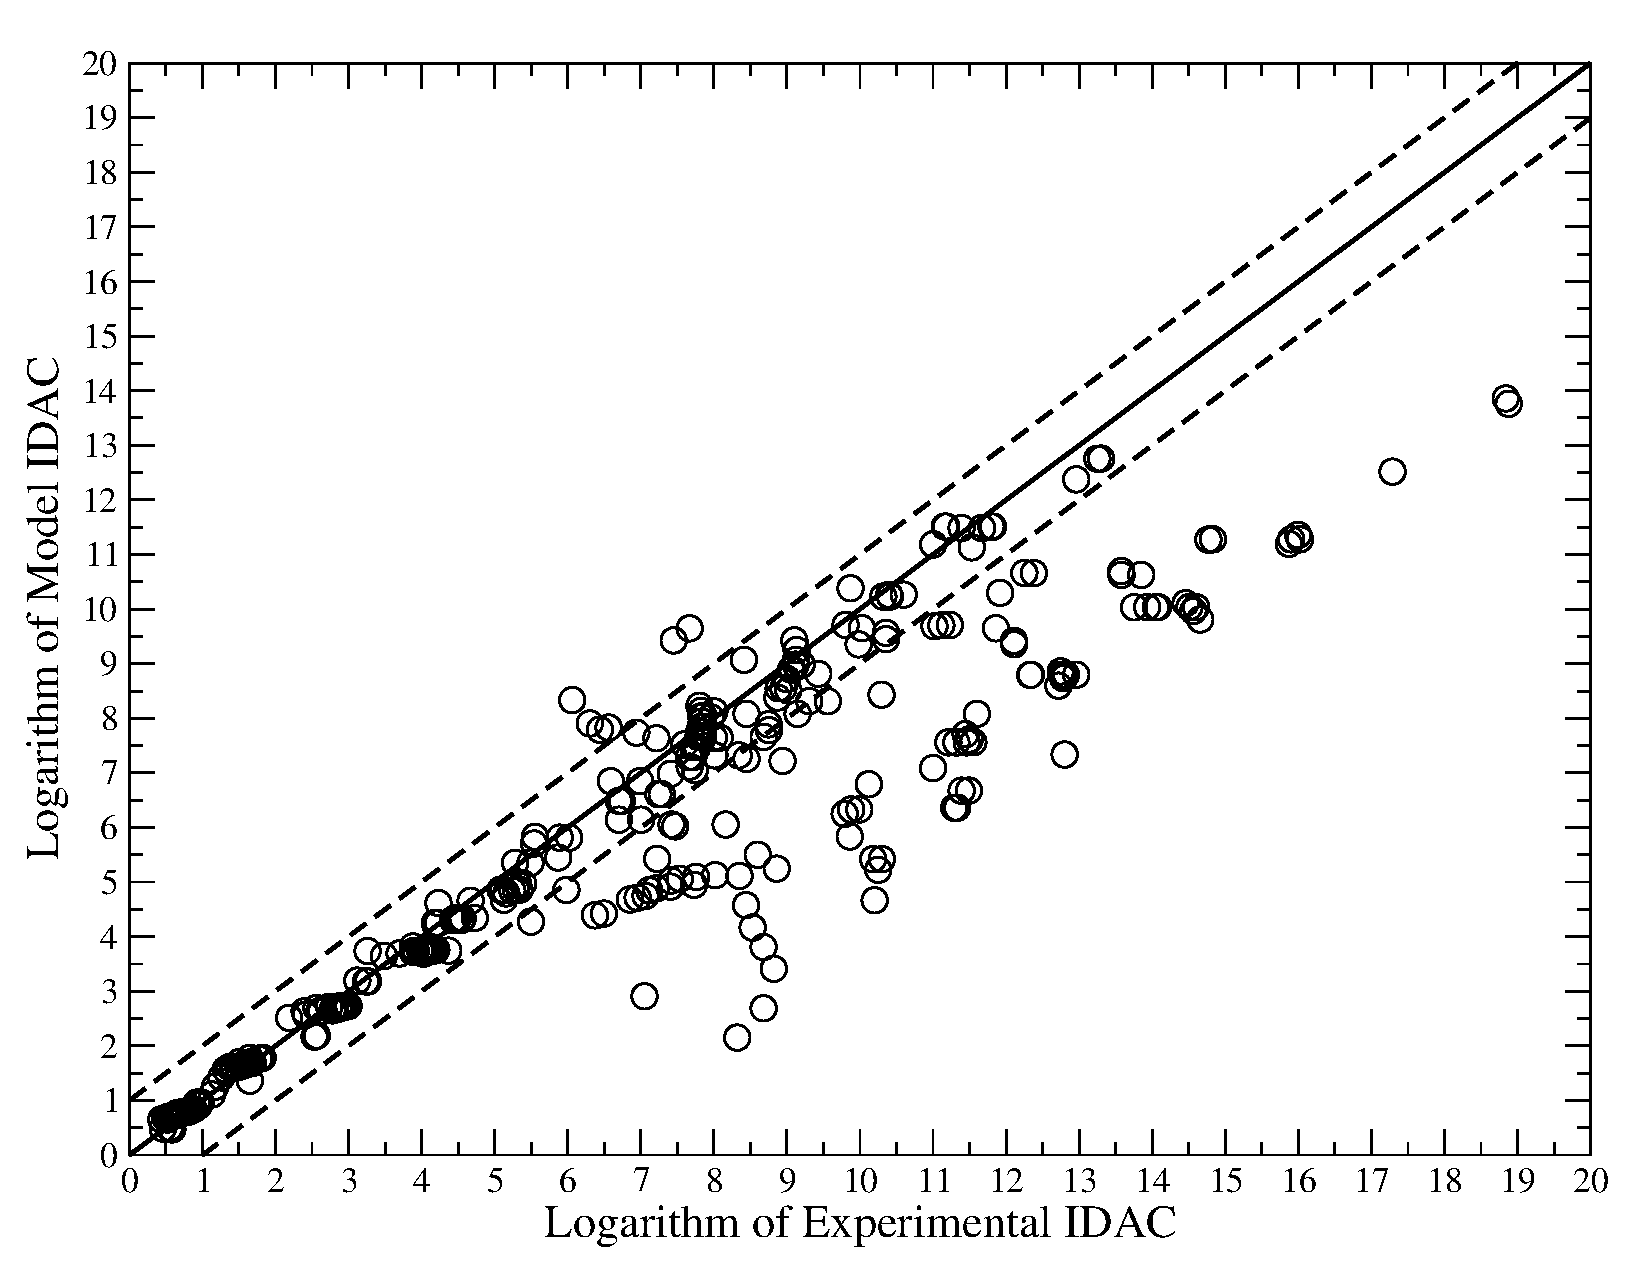
\includegraphics[width=0.4\textwidth]{Figures/IDACAq_unifac}}
\end{figure}
\scriptsize
\fullcite{SoaresFSAC2}
\end{frame}

\begin{frame}
  \frametitle{FSAC: Hydrocarbon-water mutual solubilities}

\begin{figure}
\subfigure[n-Hexane-Water] {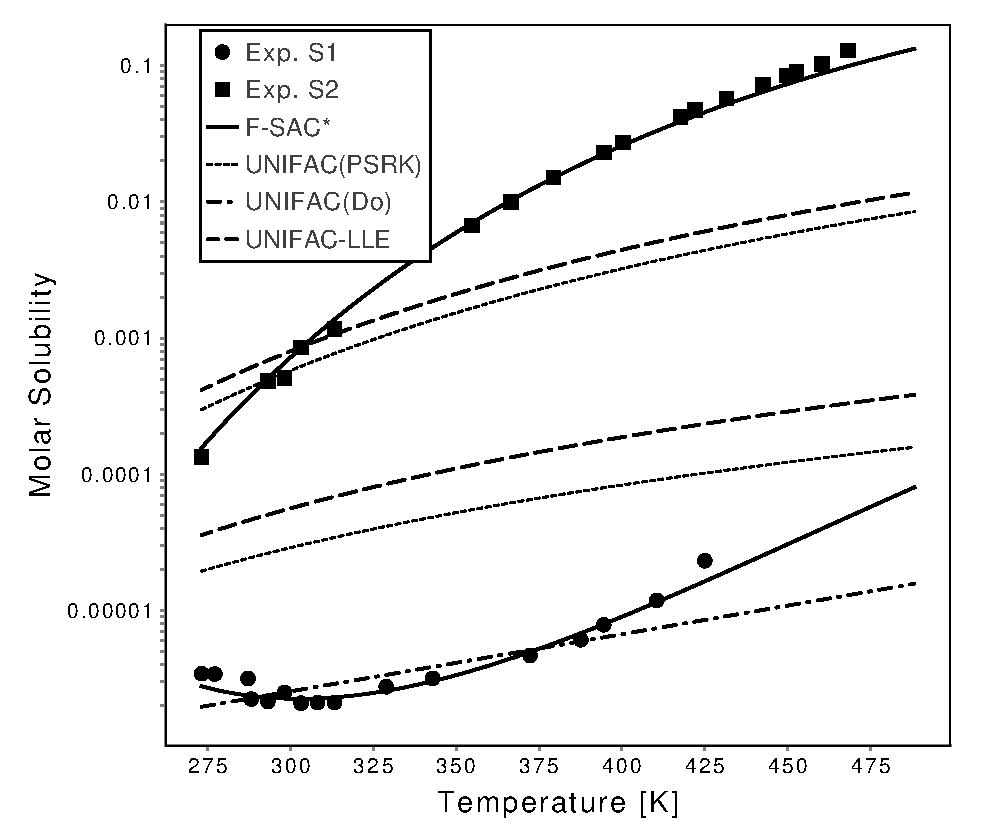
\includegraphics[width=0.4\textwidth]{Figures/N-HEXANE-WATER}}
\subfigure[Toluene-Water] {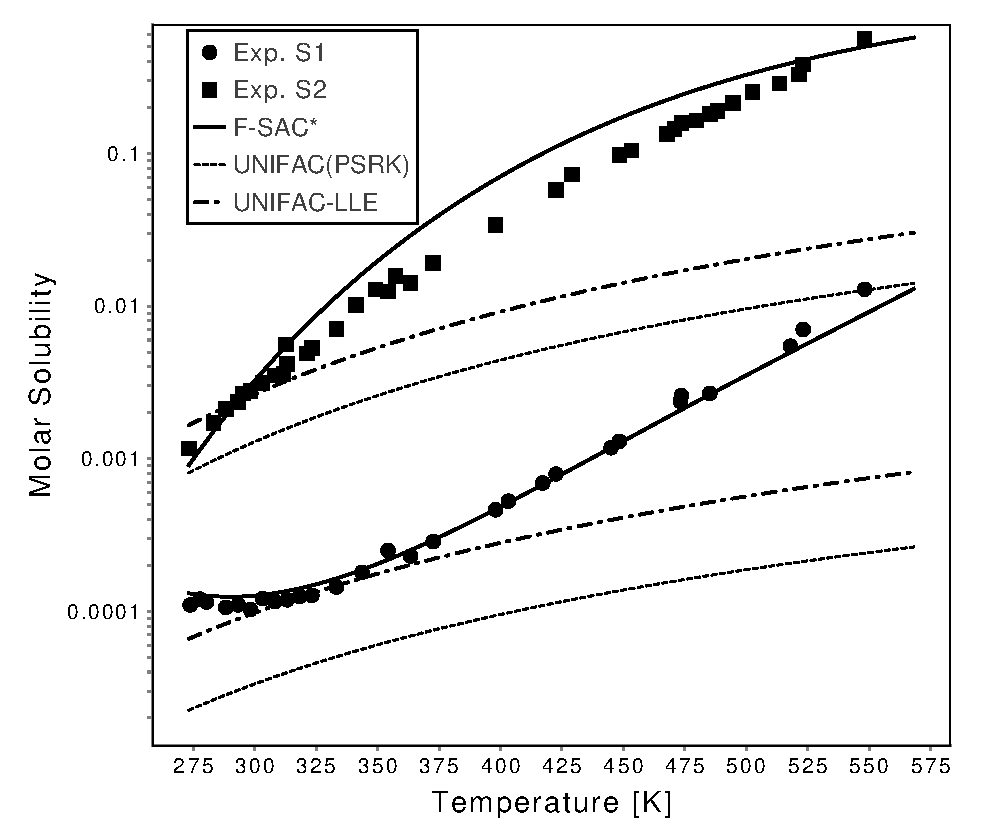
\includegraphics[width=0.4\textwidth]{Figures/TOLUENE-WATER}}
\end{figure}
\scriptsize
\fullcite{Possani:2014}
\end{frame}

% \subsection*{Wide range of temperature and pressure}

\begin{frame}[plain]
  \frametitle{Predicting high-pressure VLE with SCMR}
  \begin{itemize}
    \item The F-SAC can be combined with SRK with Mathias-Copeman $\alpha$ function and the Self-Consistent Mixing Rule\myfootcite{Staudt2012} (SCMR)
    	for propane-benzene, no parameter is adjusted for the mixture effects:
  \end{itemize}
  \begin{center}
  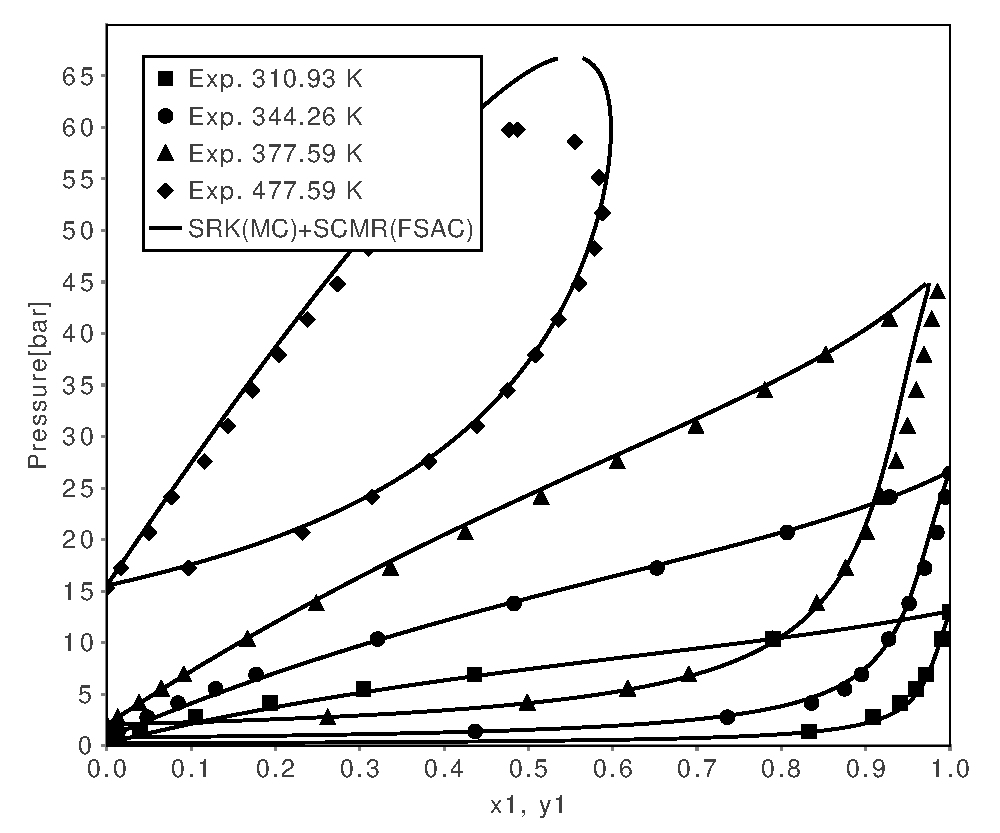
\includegraphics[width=0.5\textwidth]{Figures/PROPANE-BENZENE}
  \end{center}
\end{frame}

% \subsection*{Computational cost}
% 
% \begin{frame}
%   \frametitle{Computational cost of COSMO-based models}
%   
%   \begin{itemize}
%     \item COSMO-based models are implicit models and need a \textbf{numerical
%     method} to be \emph{solved}
%     \item The activity coefficient of the molecule $\gamma_i$ depends on the
%     activity coeffcients of the \emph{segments} $\Gamma_m$
%     (\emph{self-consistency} equation):
%   \end{itemize}
%   \begin{equation} \label{eq:iterative}
% \ln\Gamma_m =
% -\ln\left\{\sum_{_n}p_n \Gamma_n
% \exp\left[\frac{-\Delta W_{m,n}}{RT}\right]\right\}
% \end{equation}
% 
% \begin{center}
% 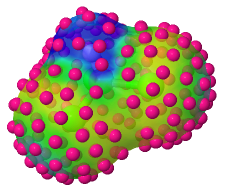
\includegraphics[width=0.3\textwidth]{Figures/ChloroformBalls}
% \end{center}
% \end{frame}
% 
% \begin{frame}[plain]
%   \frametitle{Models for simulation software need to be fast}
%   For instance the \emph{n}-butanol/water separation process suggested
%   by \fullcite{Luyben2008}:
% \begin{center}
% 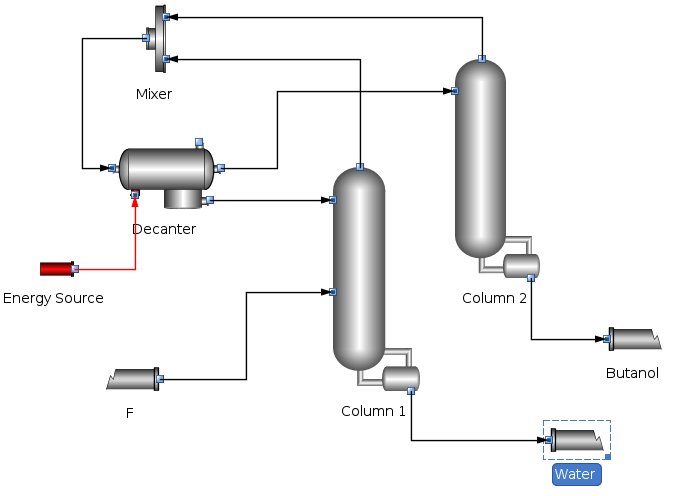
\includegraphics[width=0.8\textwidth]{Figures/ButanolWaterSeparation} \\
% \scriptsize
% Flowsheet from the \textbf{iiSE simulator} example library, 10 stages for each
% column, 3 phase separator (with stability test), 521 variables, solved in 0.3 seconds
% in an i5 laptop when using UNIFAC~(Do)
% \end{center}
% \end{frame}
% 
% 
% \begin{frame}[plain]
%   \frametitle{Models for simulation software need to be fast}
%   Or when simulating an offshore platform:
% \begin{center}
% 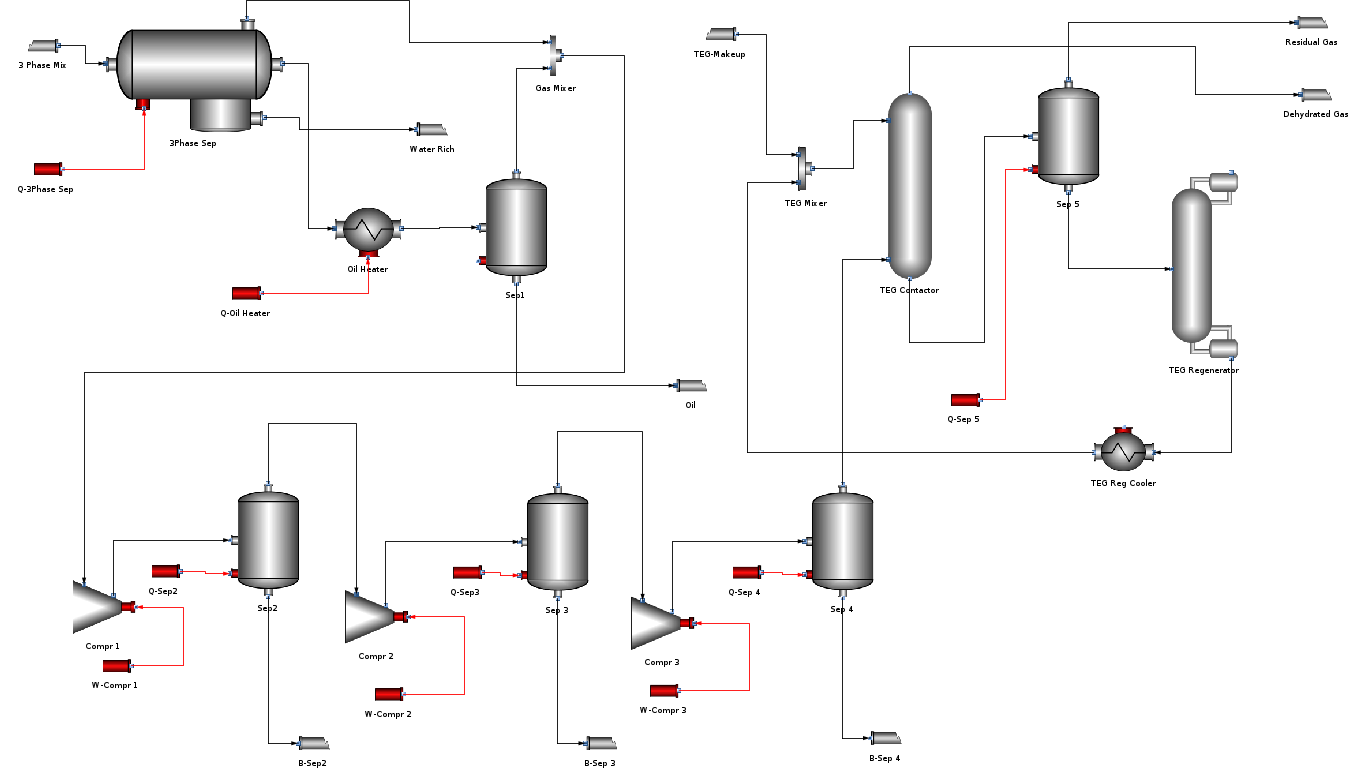
\includegraphics[width=\textwidth]{Figures/Offshore} \\
% \scriptsize
% Flowsheet from the \textbf{iiSE simulator} example library, around 2000
% variables, solved in 0.9 seconds in an i5 laptop when using
% PR+UGMR+UNIFAC~(PSRK)
% \end{center}
% \end{frame}
% 
% 
% \begin{frame}
%   \frametitle{Alternatives for fast solution of COSMO-based models}
%   
%   \begin{itemize}
%     \item Usually\myfootcite{Klamt1995,Lin2002,Grensemann2005}, the
%     self-consistency equation is solved by a successive substitution
%     method (fixed-point iteration) starting with all $\Gamma_m = 1$:
%   \end{itemize}
%   \begin{equation} \label{eq:iterative}
% \ln\Gamma_m =
% -\ln\left\{\sum_{_n}p_n \Gamma_n
% \exp\left[\frac{-\Delta W_{m,n}}{RT}\right]\right\}
% \end{equation}
% \begin{center}
% 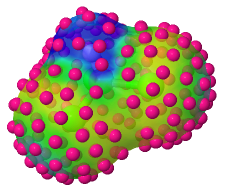
\includegraphics[width=0.3\textwidth]{Figures/ChloroformBalls}
% \end{center}
% \end{frame}
% 
% 
% \begin{frame}
%   \frametitle{Alternatives for fast solution of COSMO-based models}
%   
%   \begin{itemize}
%     \item Fixed-point iteration sounds naive\ldots
%     \item Why not a Newton-like method?
%   \end{itemize}
% \begin{center}
% \raisebox{\height}{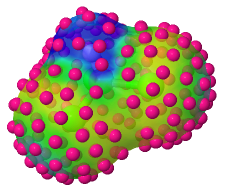
\includegraphics[width=0.25\textwidth]{Figures/ChloroformBalls}}
% 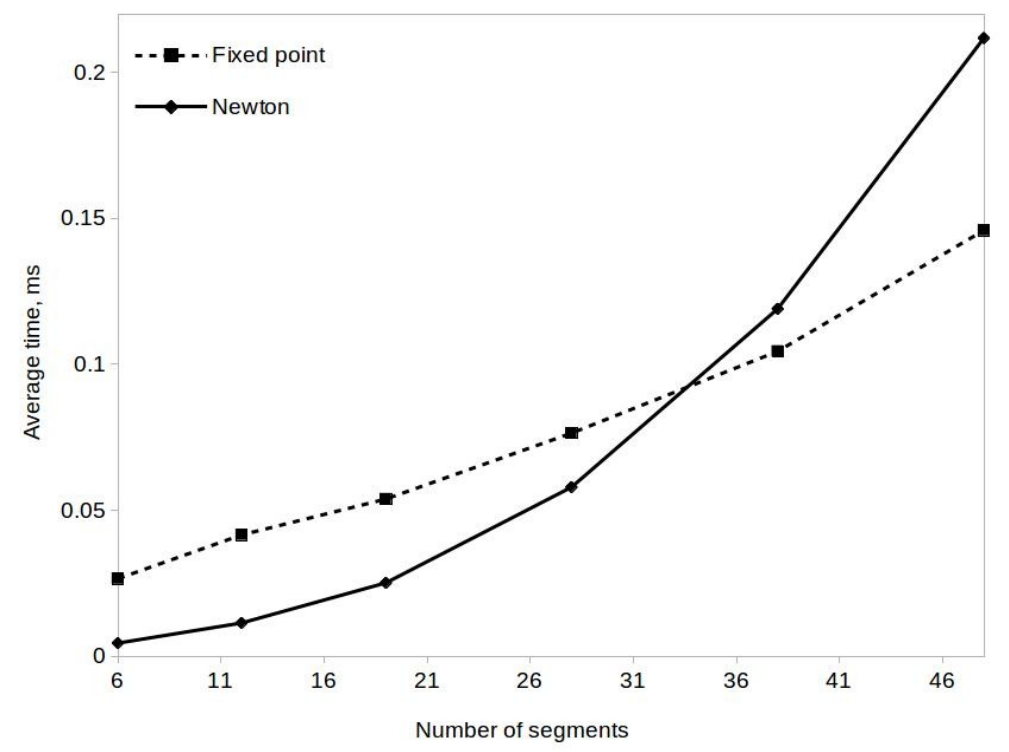
\includegraphics[width=0.7\textwidth]{Figures/Newton}
% \end{center}
% \end{frame}
% 
% \begin{frame}
% \frametitle{Newton \emph{vs.} fixed-point for COSMO-based models}
% \transdissolve
% \begin{columns}[c]
% \column{.5\textwidth}
% \begin{itemize}
%   \item Newton-like needs only 4 iterations
%   \item Fixed-point needs 12 iterations \pause
%   \item Newton-like requires $\approx 2/3 n_{seg}^3$ FLOP per iteration (LU
%   factorization)
%   \item Fixed-point requires $\approx 4 n_{seg}^2$ FLOP per iteration 
% \end{itemize}
% \column{.6\textwidth}
% 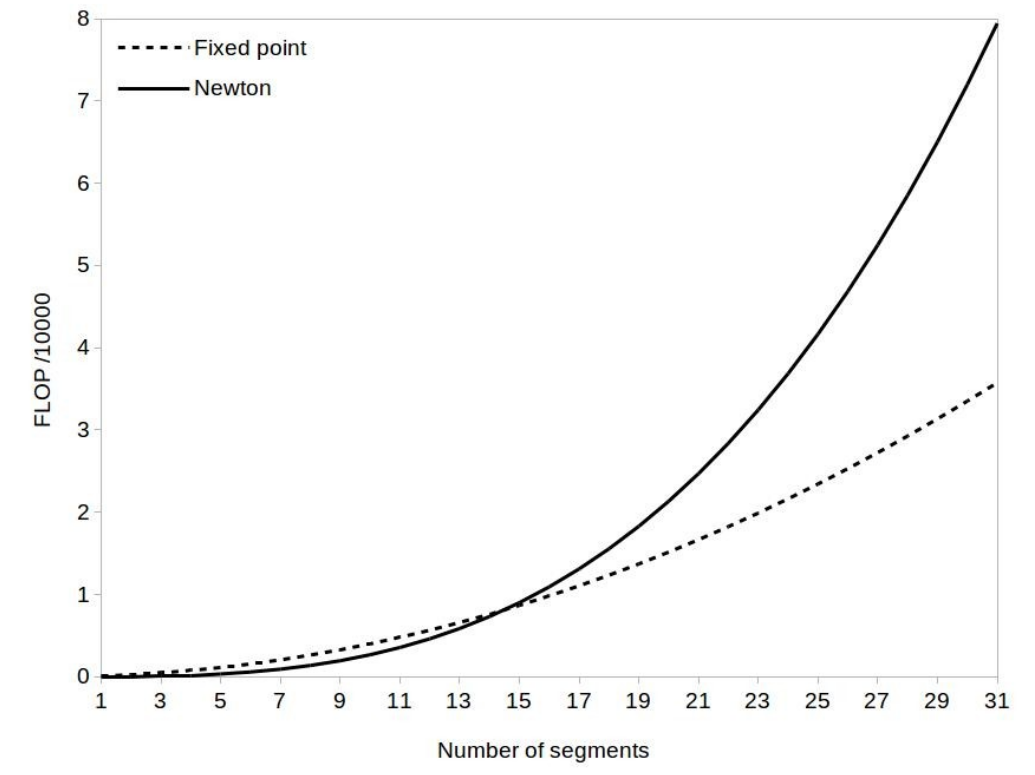
\includegraphics[width=\textwidth]{Figures/NewtonFLOP}
% \end{columns}
% \scriptsize
% \vspace{1cm}
% FLOP: floating point operations
% \end{frame}

\begin{frame}
\frametitle{Extension for electrolytes: eF-SAC}
\begin{columns}[c]
\column{.45\textwidth}
\begin{center}
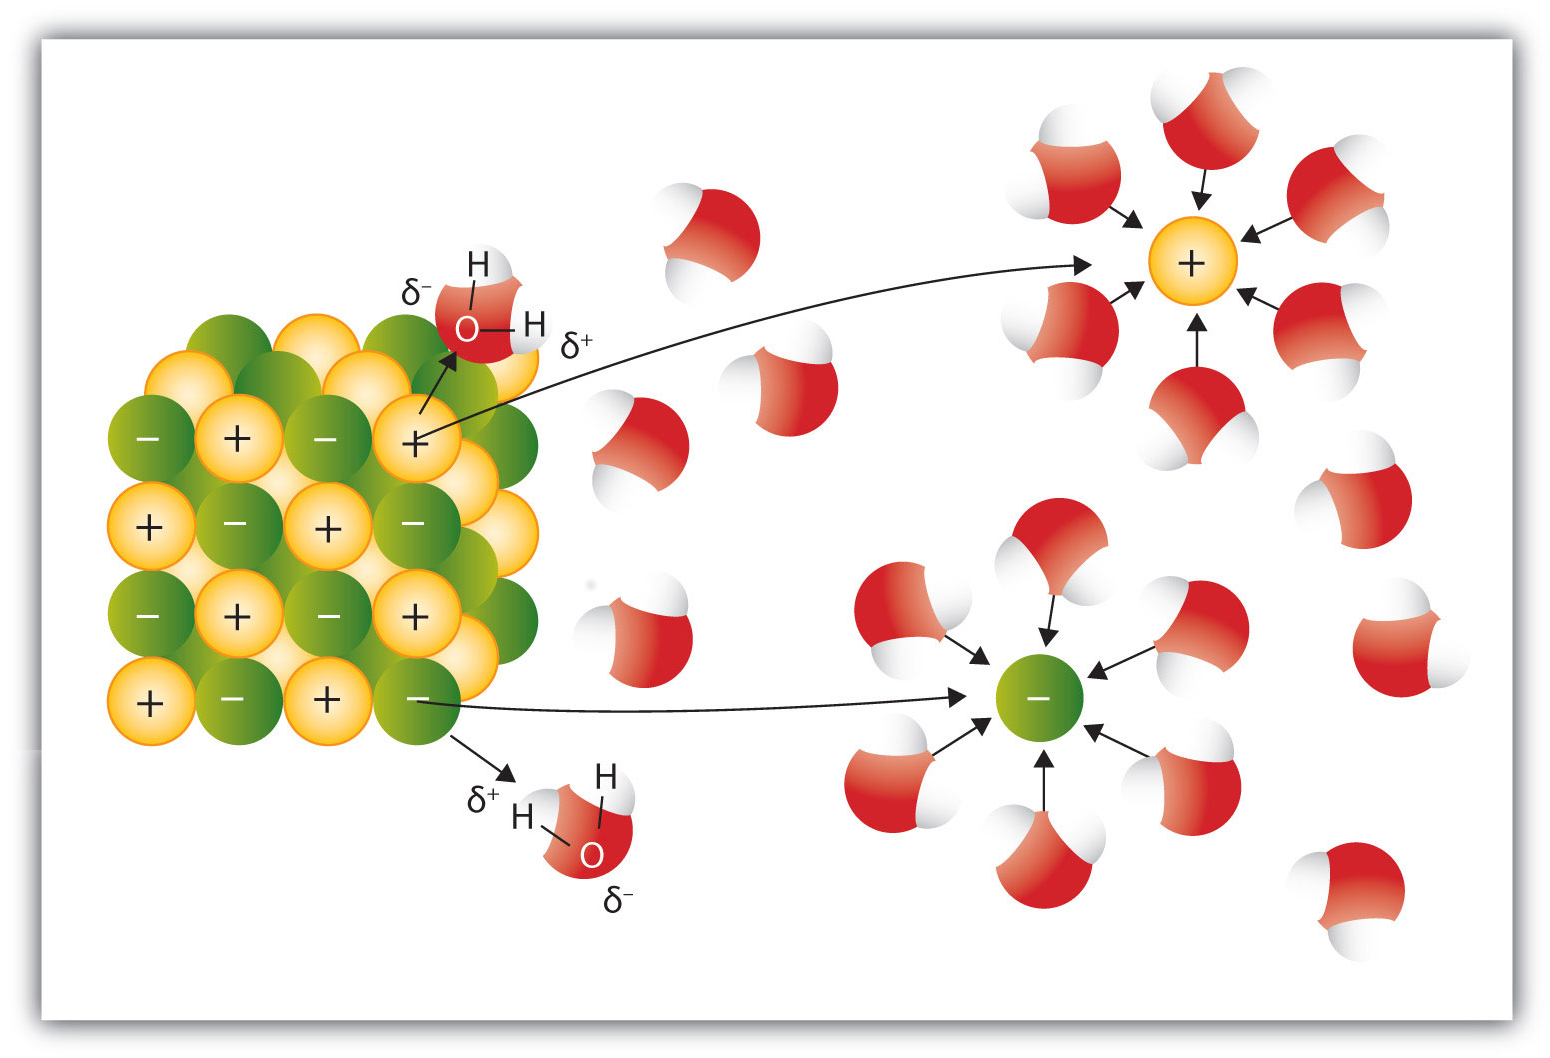
\includegraphics[width=\textwidth]{Figures/solvation.png} \\
\end{center}
\column{.65\textwidth}
\begin{itemize}
  \item Ions considered spherical with a given charge
  (+1, -1, +2, -2, etc.)
  \item Then the only parameter is the surface area (water parameters
  from previous works)
  \item To avoid direct contact between ions, their interaction energy is
  assumed high
\end{itemize}
% \begin{equation*}
% 	\ln\Gamma_m =-\ln\left[\sum_n p_n \Gamma_n
% 	\exp\left(\frac{-\Delta W_{m,n}}{RT}\right)\right]
% \end{equation*}
\end{columns}
\end{frame}

\begin{frame}
\frametitle{eF-SAC $\sigma$-profiles}
\transdissolve
\begin{columns}[c]
\column{.5\textwidth}

\begin{table}[htb]
\footnotesize 
\begin{center}
\begin{tabular}{cccc}
\hline
Group & $Q_k^+ (\text{\AA}^2)$ & $Q_k^- (\text{\AA}^2)$ &  $\sigma_k^+ (e
\text{\AA}^{-2})$\\
\hline
Li$^+$ 	& 0 & 36,96 & -0,027 \\
Na$^+$	& 0 & 29,05 & -0,034 \\
K$^+$	& 0 & 47,13 & -0,021 \\
Rb$^+$	& 0 & 40,17 & -0,025 \\
Cs$^+$	& 0 & 41,64 & -0,024 \\
F$^-$	& 27,12 & 0 &  0,037 \\
Cl$^-$	& 39,19 & 0 &  0,026 \\
Br$^-$	& 30,11 & 0 &  0,033 \\
I$^-$	& 38,69 & 0 &  0,026 \\
\hline
\end{tabular}
\end{center}
\end{table}

\column{.3\textwidth}
\includegraphics[width=0.8\textwidth]{Figures/ionicRadius}
%\includegraphics[width=0.3\textwidth]{Figures/parameters}
\end{columns}
\end{frame}

\begin{frame}
  \frametitle{Results: $\sigma$-Profile for eF-SAC}
\centering
\includegraphics[width=\textwidth]{Figures/parameters}
\end{frame}


\begin{frame}
  \frametitle{Results: $\gamma_{\pm}$}
  \begin{itemize}
    \item NaF$_{aq}$
  \end{itemize} 
\centering
\includegraphics[width=0.65\textwidth]{Figures/NaF}
\end{frame}

\begin{frame}
  \frametitle{Results: $\gamma_{\pm}$}
  \begin{itemize}
    \item LiI$_{aq}$
  \end{itemize} 
\centering
\includegraphics[width=0.65\textwidth]{Figures/LiI}
\end{frame}


\begin{frame}
  \frametitle{Results: $\gamma_{\pm}$}
  \begin{itemize}
    \item NaBr$_{aq}$
  \end{itemize} 
\centering
\includegraphics[width=0.65\textwidth]{Figures/NaBr}
\end{frame}

\begin{frame}
  \frametitle{Results: $\gamma_{\pm}$}
  \begin{itemize}
    \item LiBr$_{aq}$
  \end{itemize} 
\centering
\includegraphics[width=0.65\textwidth]{Figures/LiBr}
\end{frame}

\begin{frame}
  \frametitle{Results: $\gamma_{\pm}$}
  \begin{itemize}
    \item CsI$_{aq}$
  \end{itemize} 
\centering
\includegraphics[width=0.65\textwidth]{Figures/CsI}
\end{frame}

\section{Conclusions}
\subsection*{Conclusions}

\begin{frame}
  \frametitle{Conclusions}
  \begin{itemize}
    \item COSMO-based models have exceptional theoretical features
    \item An extensible, open, and rigorous sigma-profile database needs to be
    developed\pause
    \item Currently, results can be considered semi-quantitative
    \item Agreement with experimental data is usually obtained by
    means of empirical corrections
    \item The variation known as \textbf{F-SAC} usually produces better
    results but depends on fitted parameters \pause
    %\item Numerical efficiency is an issue for large scale process simulation
    %\pause
    \item There are certanly many other opportunities for improvement and new
    fields for application
  \end{itemize}
\end{frame}


\subsection*{Links and more info}
\frame{ %
	\frametitle{Thank you!} %
	
	\centering
	\includegraphics[width=0.3\textwidth]{TexasAMLogo} \hspace{1cm}
	\includegraphics[width=0.3\textwidth]{OryxLogo}
	
	\begin{itemize} %

	\item Molecules database at \url{http://code.google.com/p/jcosmo/}
	
	\item Download the F-SAC demonstration code at
	\url{http://www.enq.ufrgs.br/labs/lvpp}

	\item F-SAC is already available in the iiSE process simulator and being integrated
		into DWSim (open source) process simulator
	
	\item Contact: \url{rafael.pelegrini@ufrgs.br}

	\end{itemize} %
% 	\vspace{2cm}
% \includegraphics[width=\textwidth]{CBTermo2015}
} %

\end{vrpresentation}

\bibliographystyle{alpha}
\bibliography{bib.bib}

\end{document}
